\documentclass[11pt,letterpaper]{article}

\usepackage[utf8]{inputenc}
\usepackage[T1]{fontenc}
\usepackage{mathptmx}
\usepackage[margin=1in]{geometry}
\usepackage{amsmath,amssymb,bm}
\usepackage{graphicx}
\usepackage{booktabs}
\usepackage{microtype}
\usepackage{cite}
\usepackage{authblk}
\usepackage{setspace}
\usepackage{caption}
\usepackage{titlesec}
\usepackage{placeins}
\usepackage{url}
\usepackage{hyperref}
\hypersetup{
  colorlinks=true,
  linkcolor=blue,
  citecolor=blue,
  urlcolor=blue
}
\usepackage{cleveref}

% Feed IEEEtran.bst its control entry without a LaTeX \cite/\nocite warning.
\makeatletter
\AtBeginDocument{\immediate\write\@auxout{\string\citation{IEEEtran:BSTcontrol}}}
\makeatother

\setstretch{1.08}
\frenchspacing
\raggedbottom
\widowpenalty=1000
\clubpenalty=1000
\displaywidowpenalty=800

\renewcommand{\Affilfont}{\small}
\setlength{\affilsep}{0.6em}

\titlespacing*{\section}{0pt}{1.3em plus 0.2em minus 0.1em}{0.45em plus 0.06em}
\titlespacing*{\subsection}{0pt}{1.0em plus 0.15em minus 0.08em}{0.35em plus 0.05em}
\titlespacing*{\subsubsection}{0pt}{0.85em plus 0.1em minus 0.06em}{0.25em plus 0.04em}
\titlespacing*{\paragraph}{0pt}{0.75em plus 0.1em}{0.35em}

\captionsetup{
  font=small,
  labelfont=bf,
  labelsep=period,
  skip=7pt,
  justification=justified,
  singlelinecheck=false
}
\captionsetup[table]{position=above,skip=5pt}
\captionsetup[figure]{position=below,skip=8pt}

\setlength{\textfloatsep}{16pt plus 3pt minus 3pt}
\setlength{\floatsep}{12pt plus 3pt minus 2pt}
\setlength{\intextsep}{11pt plus 3pt minus 2pt}
\setlength{\abovecaptionskip}{7pt}
\setlength{\belowcaptionskip}{3pt}
\setlength{\parskip}{0.50em plus 0.12em minus 0.06em}
\setlength{\parindent}{1.2em}
\setlength{\abovedisplayskip}{7pt plus 2pt minus 2pt}
\setlength{\belowdisplayskip}{7pt plus 2pt minus 2pt}
\setlength{\abovedisplayshortskip}{4pt plus 2pt}
\setlength{\belowdisplayshortskip}{5pt plus 2pt}
\setlength{\jot}{3.5pt}

\graphicspath{{figures/}}
\newcommand{\TrueC}{9.50}
\newcommand{\TrueR}{3.60}
\newcommand{\TrueQrated}{9.00}
\newcommand{\TrueAs}{8.50}
\newcommand{\TrueRC}{34.2}
\newcommand{\TrueQC}{0.95}
\newcommand{\Ntrain}{1440}
\newcommand{\Nhold}{576}
\newcommand{\TrainDays}{5}
\newcommand{\HoldDays}{2}
\newcommand{\KnownC}{8.87}
\newcommand{\KnownR}{3.66}
\newcommand{\KnownAs}{4.53}
\newcommand{\KnownCrel}{6.6}
\newcommand{\KnownRrel}{1.8}
\newcommand{\KnownAsrel}{46.8}
\newcommand{\KnownRCrel}{4.9}
\newcommand{\KnownHoldRMSE}{0.203}
\newcommand{\KnownHoldMAE}{0.173}
\newcommand{\KnownTrainNLL}{-1.110}
\newcommand{\KnownCsd}{0.13}
\newcommand{\KnownRsd}{0.05}
\newcommand{\KnownRC}{32.5}
\newcommand{\UnknownC}{5.07}
\newcommand{\UnknownR}{6.18}
\newcommand{\UnknownQ}{4.95}
\newcommand{\UnknownAs}{3.64}
\newcommand{\UnknownCrel}{46.7}
\newcommand{\UnknownRrel}{71.5}
\newcommand{\UnknownQrel}{45.0}
\newcommand{\UnknownAsrel}{57.1}
\newcommand{\UnknownRCrel}{8.5}
\newcommand{\UnknownQCrel}{3.0}
\newcommand{\UnknownHoldRMSE}{0.113}
\newcommand{\UnknownHoldMAE}{0.092}
\newcommand{\UnknownTrainNLL}{-1.120}
\newcommand{\UnknownCsd}{1.62}
\newcommand{\UnknownRsd}{1.84}
\newcommand{\UnknownQsd}{1.59}
\newcommand{\UnknownRC}{31.3}
\newcommand{\UnknownQC}{0.98}
\newcommand{\CoolTrueC}{9.50}
\newcommand{\CoolTrueR}{3.60}
\newcommand{\CoolTrueQrated}{9.00}
\newcommand{\CoolTrueAs}{8.50}
\newcommand{\CoolTrueRC}{34.2}
\newcommand{\CoolTrueQC}{0.95}
\newcommand{\CoolNtrain}{1440}
\newcommand{\CoolNhold}{576}
\newcommand{\CoolTrainDays}{5}
\newcommand{\CoolHoldDays}{2}
\newcommand{\CoolKnownC}{9.59}
\newcommand{\CoolKnownR}{2.84}
\newcommand{\CoolKnownAs}{7.69}
\newcommand{\CoolKnownCrel}{1.0}
\newcommand{\CoolKnownRrel}{21.1}
\newcommand{\CoolKnownAsrel}{9.5}
\newcommand{\CoolKnownRCrel}{20.3}
\newcommand{\CoolKnownHoldRMSE}{0.132}
\newcommand{\CoolKnownHoldMAE}{0.109}
\newcommand{\CoolKnownTrainNLL}{-1.118}
\newcommand{\CoolKnownCsd}{0.17}
\newcommand{\CoolKnownRsd}{0.10}
\newcommand{\CoolKnownRC}{27.3}
\newcommand{\CoolUnknownC}{7.69}
\newcommand{\CoolUnknownR}{3.73}
\newcommand{\CoolUnknownQ}{7.18}
\newcommand{\CoolUnknownAs}{6.09}
\newcommand{\CoolUnknownCrel}{19.0}
\newcommand{\CoolUnknownRrel}{3.5}
\newcommand{\CoolUnknownQrel}{20.2}
\newcommand{\CoolUnknownAsrel}{28.3}
\newcommand{\CoolUnknownRCrel}{16.2}
\newcommand{\CoolUnknownQCrel}{1.5}
\newcommand{\CoolUnknownHoldRMSE}{0.174}
\newcommand{\CoolUnknownHoldMAE}{0.147}
\newcommand{\CoolUnknownTrainNLL}{-1.120}
\newcommand{\CoolUnknownCsd}{1.37}
\newcommand{\CoolUnknownRsd}{0.79}
\newcommand{\CoolUnknownQsd}{1.20}
\newcommand{\CoolUnknownRC}{28.7}
\newcommand{\CoolUnknownQC}{0.93}


\title{\textbf{A Physics-Informed Neural Stochastic Differential Equation for Building Thermal Capacity and Envelope Resistance from Smart Thermostat Runtime}}
\author[1,2]{\textbf{Sam Yang}\thanks{Correspondence: \texttt{smyng@gatech.edu}}}
\author[3,4]{\textbf{Jessica Moorefield}}
\affil[1]{Center for Advanced Power Systems, Florida State University, Tallahassee, FL 32310, USA}
\affil[2]{College of Computing, Georgia Institute of Technology, Atlanta, GA 30332, USA}
\affil[3]{Department of Computer Science, North Carolina State University, Raleigh, NC 27695, USA}
\affil[4]{Department of Computer Science and Department of English, Florida State University, Tallahassee, FL 32306, USA}

\date{\today}

\begin{document}
\maketitle
\vspace{-2.0em}

\begin{abstract}
\noindent
Accelerating the decarbonization of residential buildings and unlocking grid-scale demand flexibility require accurate estimation of thermal dynamics, specifically effective lumped thermal capacitance $C$ and envelope thermal resistance $R$. Classical gray-box identification relies on continuous-time stochastic differential equations (SDEs) fitted via Kalman maximum likelihood, whereas recent physics-informed neural network (PINN) formulations minimize deterministic energy-balance residuals. However, both paradigms make assumptions at odds with commercial smart-thermostat telemetry: they assume metered thermal power and instantaneous point-sampled temperatures, whereas thermostats report interval runtime and time-averaged indoor temperatures ($\bar{y}_k$). We encode runtime as a signed fraction $u \in [-1, 1]$ ($u>0$ heating, $u<0$ cooling). Here, we formulate a physics-informed neural SDE (PIN-SDE) that integrates a lumped energy-balance drift, a latent Ornstein--Uhlenbeck (OU) occupancy process, a left-endpoint interval-mean Kalman measurement operator, and an identifiability-regularized neural remainder, trained end-to-end in JAX via automatic differentiation through the Kalman path likelihood. We evaluate parameter identifiability on paired seven-day winter-heating and summer-cooling digital twins using a strict chronological two-day holdout. When HVAC capacity $Q_\mathrm{rated}$ is known a priori, MAP $C$ is within $\KnownCrel$\% (heating) and $\CoolKnownCrel$\% (cooling) of plant truth; metered cooling does \emph{not} recover $R$ ($\CoolKnownRrel$\%). When restricted to observed runtime alone, $C$ and $Q_\mathrm{rated}$ alias in both seasons (relative errors $\UnknownCrel$\% / $\CoolUnknownCrel$\% on $C$ and $\UnknownQrel$\% / $\CoolUnknownQrel$\% on $Q_\mathrm{rated}$); winter also inflates $R$ by $\UnknownRrel$\%. The ratio $Q_\mathrm{rated}/C$ stays closer to truth ($\UnknownQCrel$\% heating, $\CoolUnknownQCrel$\% cooling) than $C$ or $Q_\mathrm{rated}$ separately. Runtime-only holdout open-loop temperature RMSE remains low in both seasons ($\UnknownHoldRMSE\,\mathrm{K}$ heating, $\CoolUnknownHoldRMSE\,\mathrm{K}$ cooling), so indoor temperature fit---even in out-of-sample forward rollouts---is an unreliable surrogate for physical parameter identification. These results illustrate observability limits of runtime-only identification on these twins and provide an open-source JAX implementation.
\end{abstract}

\vspace{0.2em}
\noindent\textbf{Keywords:} building thermal identification; gray-box stochastic differential equations; physics-informed neural networks; smart thermostat runtime; parameter identifiability; uncertainty quantification.
\vspace{0.75em}

\section{Introduction}
\label{sec:intro}

Buildings account for over 30\% of global final energy consumption and a commensurate share of greenhouse gas emissions, with space heating and cooling representing the dominant end-use~\cite{reynders2014,deconinck2016}. Harnessing buildings as distributed energy resources for grid-interactive efficient buildings (GEBs), automated demand response, and model predictive control (MPC) requires accurate, low-order thermal models~\cite{gokhale2022,chen2023physcon}. At the core of low-order lumped building models are two governing physical parameters: the effective lumped thermal capacitance $C$ ($\mathrm{kWh/K}$), capturing the aggregate thermal storage of indoor air and internal mass, and the effective envelope thermal resistance $R$ ($\mathrm{K/kW}$), capturing overall envelope transmission and infiltration losses ($UA = 1/R$). Spatially resolved 3D volume-element models can simulate indoor temperature and humidity fields from envelope geometry and local energy balances~\cite{yang2018vem}; operational identification from thermostat telemetry instead requires this lumped $(C,R)$ description. Accurate knowledge of $(C, R)$ is essential not only for multi-hour thermal load forecasting, but also for evaluating building retrofit efficacy, verifying insulation quality, and scheduling flexible heating, ventilation, and air conditioning (HVAC) operation without compromising occupant comfort~\cite{bacher2011,rouchier2018}.

For decades, the standard paradigm for continuous-time building identification has been the stochastic gray-box resistance-capacitance (RC) framework developed by Madsen, Holst, Bacher, and collaborators~\cite{madsen1995,andersen2000,kristensen2004,bacher2011,thilker2021,jimenez2008}. Formulated as stochastic differential equations (SDEs) and implemented in toolboxes such as CTSM-R, these models introduce Wiener diffusion processes to capture unmeasured internal heat gains, stochastic solar infiltration, and microclimatic variability. Model parameters are typically estimated via maximum likelihood through continuous-discrete Kalman or extended Kalman filtering~\cite{kristensen2004,sarkka2013}. Parallel to gray-box methods, the emergence of physics-informed neural networks (PINNs)~\cite{raissi2019} and neural differential equations~\cite{chen2018node,li2020sde,kidger2021sde} has motivated hybrid building models that augment deterministic thermal circuits with deep neural network residuals or train neural ODEs to invert envelope parameters from sensor time series~\cite{gokhale2022,chen2023physcon,dinatale2022,sievers2023,kim2025,liu2025etp}.

Despite their theoretical maturity, existing gray-box and physics-informed identification frameworks suffer from two fundamental disconnects when deployed on commercial smart-thermostat data (e.g., ecobee, Google Nest, Honeywell):
\begin{enumerate}
\item \textbf{Unmetered HVAC power versus observed runtime duty cycle:} Canonical gray-box and PINN formulations assume an explicitly metered heat flux input $\Phi_h(t)$ (in kW)~\cite{madsen1995,kristensen2004,gokhale2022}. In residential reality, smart thermostats record interval runtime (duty cycle or compressor seconds) rather than delivered cooling/heating power~\cite{huchuk2021}. We encode that runtime as a signed fraction $u \in [-1, 1]$: $u>0$ while heating, $u<0$ while cooling, and heating-only exports use $u \in [0, 1]$. The runtime fraction is observed; the actual HVAC capacity $Q_\mathrm{rated}$ (in kW) is unmeasured and varies with equipment sizing, duct degradation, and ambient operating conditions.
\item \textbf{Instantaneous sampling versus interval-averaged telemetry:} Standard Kalman filter formulations assume instantaneous Dirac point observations $Y_k = T(t_k) + e_k$. However, smart thermostats log aggregate statistics, specifically the time-average indoor temperature $\bar{y}_k = \frac{1}{\Delta}\int_{t_{k-1}}^{t_k} T(s)\,ds$ over the interval $\Delta$~\cite{huchuk2021}. Disregarding this integrated observation operator introduces discretization bias and degrades parameter estimation accuracy.
\end{enumerate}

Furthermore, unmeasured occupant behavior and internal appliance gains ($Q_\mathrm{int}$) create strong low-frequency disturbances that can corrupt envelope resistance estimates if treated merely as Gaussian white noise~\cite{rouchier2018}. When neural network residuals are introduced to compensate for unmodeled dynamics, they frequently suffer from parameter leakage: unconstrained neural networks can freely absorb envelope conductance $UA$ or heating gain $1/C$, destroying the physical interpretability of the identified parameters~\cite{dinatale2022}.

\begin{table}[t]
\caption{\textbf{Scope of building thermal identification paradigms} relative to the proposed physics-informed neural SDE framework. The comparison highlights dynamic formulation, HVAC input representation, observation operator, and residual structure.}
\label{tab:prior}
\centering
\small
\begin{tabular}{@{}p{0.24\textwidth}p{0.22\textwidth}p{0.24\textwidth}p{0.22\textwidth}@{}}
\toprule
\textbf{Framework} & \textbf{Dynamics \& Noise} & \textbf{HVAC \& Temperature Obs.} & \textbf{Neural Remainder / UQ} \\
\midrule
Madsen \& Holst; Bacher \& Madsen~\cite{madsen1995,bacher2011} & Parametric RC SDE; Wiener process noise & Metered heat flux $\Phi_h$; Point sample $T(t_k)$ & None; Fisher information MLE covariance \\
CTSM-R / Kristensen et al.~\cite{kristensen2004} & Gray-box SDE; Continuous-discrete EKF & Exogenous metered power; Point sample $Y_k$ & None; Laplace asymptotic standard errors \\
Gokhale et al.; Kim et al.; Liu et al.~\cite{gokhale2022,kim2025,liu2025etp} & Deterministic RC ODE / PINN & Thermostat temperature; Assumed/known $Q_\mathrm{hvac}$ & Deterministic NN residual; No formal SDE UQ \\
Sievers et al.; Di Natale et al.~\cite{sievers2023,dinatale2022} & Hybrid RC ODE + NN in JAX / PyTorch & Simulated or metered power & Unconstrained or PCNN; Deterministic rollout loss \\
\textbf{This Work (PIN-SDE)} & \textbf{RC SDE + Latent OU occupancy} & \textbf{Observed signed runtime $u$; Left-endpoint interval-mean $\bar{y}_k$} & \textbf{Two-stage identifiability penalty; Train sum-NLL Laplace (FD Hessian)} \\
\bottomrule
\end{tabular}
\end{table}

In this paper, we address these challenges by developing an end-to-end, differentiable physics-informed neural stochastic differential equation (PIN-SDE) framework tailored specifically to smart-thermostat telemetry. Our formulation incorporates:
\begin{itemize}
\item A continuous-time lumped thermal energy-balance SDE with an unobserved Ornstein--Uhlenbeck (OU) latent occupancy process whose identifier mean is a daily Fourier series;
\item A linear-Gaussian Kalman filter on an Euler--Maruyama discretization that observes the left-endpoint interval-mean indoor temperature (not a Dirac sample at $t_k$);
\item A signed runtime formulation $Q_\mathrm{hvac} = Q_\mathrm{rated}u$ ($u \in [-1, 1]$) supporting heating and cooling, with $Q_\mathrm{rated}$ either supplied via metered kW or learned;
\item A two-stage training scheme with an identifiability regularizer that penalizes remainder correlation with $(T_a - T)$, solar irradiance $I$, and the HVAC channel;
\item A strictly causal evaluation protocol: chronological holdout open-loop \emph{mean} Euler--Maruyama rollout (process noise set to zero), plus a finite-difference Laplace approximation of the train sum-NLL MAP Hessian with neural weights held at MAP.
\end{itemize}

Using paired digital-twin benchmarks spanning a seven-day winter heating period and a seven-day summer cooling period, we run the same known-HVAC-capacity versus runtime-only comparison in both seasons. Metered thermal power recovers $C$ more accurately than runtime alone in both seasons ($\KnownCrel$\% vs.\ $\UnknownCrel$\% heating; $\CoolKnownCrel$\% vs.\ $\CoolUnknownCrel$\% cooling). It also recovers winter $R$ ($\KnownRrel$\% vs.\ $\UnknownRrel$\%), but \emph{not} summer $R$: known-kW $R$ error is $\CoolKnownRrel$\% against $\CoolUnknownRrel$\% for runtime-only, consistent with a summer $UA$--$A_s$ trade-off. Runtime-only still induces a $Q_\mathrm{rated}$--$C$ scaling valley in both seasons ($\UnknownCrel$\% / $\UnknownQrel$\% heating; $\CoolUnknownCrel$\% / $\CoolUnknownQrel$\% cooling). In winter the runtime fit also inflates $R$ by $\UnknownRrel$\%, yet its holdout open-loop RMSE ($\UnknownHoldRMSE\,\mathrm{K}$) is lower than the metered-power RMSE ($\KnownHoldRMSE\,\mathrm{K}$). In summer, stronger solar excitation improves unknown-protocol $R$ and $A_s$ relative to winter, while $C$ and $Q_\mathrm{rated}$ still scale together and holdout RMSE remains $\CoolUnknownHoldRMSE\,\mathrm{K}$. Indoor temperature tracking is therefore insufficient to validate physical parameter recovery. Table~\ref{tab:prior} summarizes the scope of the proposed method and compares it against existing approaches in the literature.

\section{Mathematical Formulation}
\label{sec:model}

\subsection{Physical System Scope and Assumptions}
\label{sec:model-scope}
We consider a single-zone lumped thermal representation of a residential building. The system state is defined by the effective indoor air and lumped mass temperature $T(t)$ ($^\circ\mathrm{C}$) and an unmeasured latent internal gain state $Q_\mathrm{int}(t)$ ($\mathrm{kW}$). All physical equations are formulated consistently with time $t$ in hours ($\mathrm{h}$), thermal capacitance $C$ in $\mathrm{kWh/K}$, thermal resistance $R$ in $\mathrm{K/kW}$, and heat fluxes in $\mathrm{kW}$. Under this dimensional convention, the thermal accumulation term $C\,\frac{dT}{dt}$ has units of power ($\mathrm{kW}$).

The physical boundary exchanges include envelope transmission and infiltration losses, direct and diffuse solar gains through an effective solar aperture $A_s$ ($\mathrm{m}^2$), latent moisture coupling parameterized by $\beta$ ($\mathrm{kW}$ per $\mathrm{kg_w\,kg_{da}}^{-1}$), HVAC heating or cooling load $Q_\mathrm{hvac}(t)$ ($\mathrm{kW}$), unmeasured internal occupancy and appliance gains $Q_\mathrm{int}(t)$, and an exogenous neural remainder $r_\theta(\bm{u})$ capturing unmodeled dynamics.

\subsection{Coupled Energy-Balance Neural SDE}
\label{sec:model-sde}
The continuous-time system dynamics are governed by the two-dimensional Ito stochastic differential equation:
\begin{align}
\label{eq:sdeT}
dT(t) &= \frac{1}{C}\Bigl[ U(t)A_\mathrm{eff}\bigl(T_a(t) - T(t)\bigr) + A_s I(t) + \beta\bigl(\omega_a(t) - \omega_i(t)\bigr) + Q_\mathrm{hvac}(t) + Q_\mathrm{int}(t) + r_\theta\bigl(\bm{u}(t)\bigr) \Bigr]dt \nonumber \\
&\quad + \sigma_T\bigl(\bm{u}(t)\bigr)\,dW_T(t), \\
\label{eq:sdeQ}
dQ_\mathrm{int}(t) &= \kappa\bigl(\mu(t) - Q_\mathrm{int}(t)\bigr)\,dt + \sigma_q\,dW_Q(t),
\end{align}
where $W_T(t)$ and $W_Q(t)$ are mutually independent standard Brownian motion processes. The physical components and parameters are defined as follows:
\begin{itemize}
\item \textbf{Wind-Dependent Envelope Conductance:} The effective envelope conductance $UA_\mathrm{eff}(t)$ ($\mathrm{kW\,K}^{-1}$) incorporates wind-induced infiltration and surface convection:
\begin{equation}
\label{eq:ua-eff}
U(t)A_\mathrm{eff} = \frac{1}{R}\bigl(1 + k_v v_\mathrm{wind}(t)\bigr),
\end{equation}
where $v_\mathrm{wind}(t)$ is the local wind speed ($\mathrm{m/s}$) and $k_v = 0.04\,\mathrm{s/m}$ is a fixed empirical wind coupling coefficient~\cite{bacher2011}.
\item \textbf{Solar and Moisture Gains:} $I(t)$ is the global horizontal solar irradiance ($\mathrm{kW/m^2}$; GHI in $\mathrm{W/m^2}$ divided by $1000$). Humidity ratios $\omega_a, \omega_i$ ($\mathrm{kg_w/kg_{da}}$) are computed from dry-bulb temperature and relative humidity via Magnus--Tetens psychrometrics at atmospheric pressure $P_\mathrm{atm}=101{,}325\,\mathrm{Pa}$:
\begin{align}
\label{eq:psych}
P_\mathrm{sat}(T) &= 610.94 \exp\left( \frac{17.625\,T}{T + 243.04} \right) \quad (\mathrm{Pa}), \qquad P_v = \min\bigl(\mathrm{RH}\cdot P_\mathrm{sat}(T),\; 0.95\,P_\mathrm{atm}\bigr), \\
\omega(T, \mathrm{RH}) &= 0.62198 \left( \frac{P_v}{P_\mathrm{atm} - P_v} \right) \quad (\mathrm{kg_w\,kg_{da}}^{-1}),
\end{align}
with $\mathrm{RH} \leftarrow \mathrm{clip}(\mathrm{RH},\,10^{-4},\,0.999)$. These enter the identifier as interval-constant series. The digital twin holds indoor RH at $0.40$ and evaluates $\omega_i$ from the plant indoor temperature at each 1-minute step; the filter does not recompute $\omega_i$ from the Kalman mean $T$.
\item \textbf{HVAC Actuation and Runtime:} In the realistic thermostat setting, the delivered thermal (cooling/heating) power is parameterized as:
\begin{equation}
\label{eq:qhvac}
Q_\mathrm{hvac}(t) = Q_\mathrm{rated} u(t),
\end{equation}
where $u(t) \in [-1, 1]$ is the signed observed runtime fraction ($u > 0$ for heating, $u < 0$ for cooling), and $Q_\mathrm{rated} > 0$ ($\mathrm{kW}$) is the positive rated thermal capacity. In the optimistic baseline protocol, $Q_\mathrm{hvac}(t)$ is provided as a known metered heat flux and $Q_\mathrm{rated}$ is not updated.
\item \textbf{Latent Occupancy Process:} $Q_\mathrm{int}(t)$ evolves as a mean-reverting Ornstein--Uhlenbeck (OU) process with reversion rate $\kappa$ ($\mathrm{h}^{-1}$) and diffusion coefficient $\sigma_q$ ($\mathrm{kW/h^{0.5}}$). On the \emph{identifier}, the time-varying mean $\mu(t)$ is a positive $K=3$ Fourier series:
\begin{equation}
\label{eq:fourier-occ}
\mu(t) = \mathrm{softplus}\Biggl( a_0 + \sum_{k=1}^{3} \Bigl[ a_k \sin\Bigl(\frac{2\pi k t}{24}\Bigr) + b_k \cos\Bigl(\frac{2\pi k t}{24}\Bigr) \Bigr] \Biggr).
\end{equation}
The digital-twin \emph{plant} instead mean-reverts to a diurnal schedule of Gaussian occupancy bumps (Section~\ref{sec:results-setup}); the Fourier $\mu(t)$ is therefore misspecified relative to the plant.
\item \textbf{Neural Remainder and Diffusion:} Let $\bm{z}_k$ be the train-prefix $z$-scored exogenous feature vector
\begin{equation}
\label{eq:features}
\bm{u}_k = \bigl[T_a,\; I,\; \mathrm{RH}_a,\; v_\mathrm{wind},\; \mathrm{HVAC}_k,\; \sin\omega_k,\; \cos\omega_k,\; \sin 2\omega_k,\; \cos 2\omega_k\bigr]^\top,
\end{equation}
with $\omega_k = 2\pi t_k/24$ and $\mathrm{HVAC}_k$ equal to signed runtime $u_k$ in unknown-$Q_\mathrm{rated}$ mode or metered $Q_\mathrm{hvac}$ in known-kW mode. Indoor $T$ and $Q_\mathrm{int}$ are excluded so the conditional filter remains linear-Gaussian in the state. With gate $g=0$ in Stage~A and $g=1$ thereafter,
\begin{align}
\label{eq:remainder-net}
r_\theta(\bm{u}_k) &= g\cdot 0.18\,\tanh\bigl(\mathrm{MLP}_{16,16}(\bm{z}_k)\bigr), \\
\label{eq:sigma-net}
\sigma_T(\bm{u}_k) &= \sigma_T^{\mathrm{base}}\exp\Bigl(\tfrac12 g\cdot 0.35\,\mathrm{clip}\bigl(\mathrm{MLP}_{8,8}(\bm{z}_k),-2,2\bigr)\Bigr).
\end{align}
Hidden layers use $\tanh$; last-layer weights of both nets are initialized at zero. The scalar $\sigma_T^{\mathrm{base}}$ is the shifted-softplus noise parameter in~\eqref{eq:sdeT}.
\end{itemize}

\subsection{Continuous-Discrete Interval-Average Kalman Likelihood}
\label{sec:model-obs}
Smart thermostats report measurements aggregated over the telemetry interval $\Delta = t_k - t_{k-1}$ (here $\Delta = 5\,\mathrm{min} = 1/12\,\mathrm{h}$). The continuous-time observation model is the interval mean
\begin{equation}
\label{eq:obs}
\bar{y}_k = \frac{1}{\Delta}\int_{t_{k-1}}^{t_k} T(s)\,ds + e_k, \qquad e_k \sim \mathcal{N}(0, \sigma_y^2),
\end{equation}
with sensor noise $\sigma_y$ ($\mathrm{K}$). The identifier does not evaluate this integral in continuous time. Each reporting interval is split into $n_\mathrm{sub}=5$ Euler--Maruyama substeps of duration $\delta t = \Delta/n_\mathrm{sub} = 1\,\mathrm{min} = 1/60\,\mathrm{h}$, with weather, HVAC, remainder, and $\sigma_T(\bm{u})$ held constant (zero-order hold) on the interval. An accumulator $S$ stores the sum of left-endpoint indoor temperatures, $S' = S + T$, so after $n_\mathrm{sub}$ steps the predicted measurement is the discrete left-endpoint mean $\hat{y}_k = S/n_\mathrm{sub}$. The augmented state $\bm{x} = [T, Q_\mathrm{int}, S]^\top$ evolves as
\begin{equation}
\label{eq:augmented-em}
\bm{x}_{m} = \bm{F}_3 \bm{x}_{m-1} + \bm{g}_3 + \bm{w}_m, \qquad \bm{w}_m \sim \mathcal{N}(\bm{0}, \bm{Q}_d),
\end{equation}
with
\begin{equation}
\label{eq:F3}
\bm{F}_3 = \begin{bmatrix} 1 - \delta t \frac{UA_\mathrm{eff}}{C} & \frac{\delta t}{C} & 0 \\ 0 & 1 - \delta t\,\kappa & 0 \\ 1 & 0 & 1 \end{bmatrix}, \qquad
\bm{g}_3 = \begin{bmatrix} \frac{\delta t}{C}\Bigl( UA_\mathrm{eff}T_a + A_s I + \beta(\omega_a - \omega_i) + Q_\mathrm{hvac} + r_\theta(\bm{u}_k) \Bigr) \\ \delta t\,\kappa\,\mu(t_k) \\ 0 \end{bmatrix},
\end{equation}
\begin{equation}
\bm{Q}_d = \begin{bmatrix} \delta t\,\sigma_T(\bm{u}_k)^2 & 0 & 0 \\ 0 & \delta t\,\sigma_q^2 & 0 \\ 0 & 0 & 0 \end{bmatrix}.
\end{equation}
The observation row is $\bm{H} = [0, 0, 1/n_\mathrm{sub}]$, so $\hat{y}_k = \bm{H}\bm{x}(t_k\mid t_{k-1})$ and $S_k = \bm{H}\bm{P}(t_k\mid t_{k-1})\bm{H}^\top + \sigma_y^2$. A Joseph-stabilized scalar measurement update is applied; $[T, Q_\mathrm{int}]^\top$ is forwarded and $S$ is reset to zero. Training uses the Gaussian path NLL on the train prefix,
\begin{equation}
\label{eq:nll}
\mathcal{L}_\mathrm{NLL}(\bm{\Theta}) = \frac{1}{2}\sum_{k=1}^{N_\mathrm{train}} \Bigl[ \ln(2\pi S_k) + \frac{(\bar{y}_k - \hat{y}_k)^2}{S_k} \Bigr].
\end{equation}
The optimizer minimizes the \emph{mean} interval NLL $\mathcal{L}_\mathrm{NLL}/N_\mathrm{train}$ plus regularizers; Laplace UQ uses the equivalent sum $N_\mathrm{train}$ times that mean objective.

\section{Identifiability Analysis and Estimation Framework}
\label{sec:id}

\subsection{Structural and Practical Identifiability under On/Off Excitation}
\label{sec:id-analysis}
A central theoretical question in building thermal identification is whether $(C, R, Q_\mathrm{rated})$ can be uniquely resolved from closed-loop thermostat time series. Neglecting wind inflation, moisture, and the neural remainder, the energy-balance ODE during active heating ($u = 1$), active cooling ($u = -1$), and idle/off ($u = 0$) is:
\begin{align}
\label{eq:id-heating}
\text{Heating } (u=1): \quad &\frac{dT}{dt} = \frac{Q_\mathrm{rated}}{C} - \frac{1}{RC}(T - T_a) + \frac{A_s I + Q_\mathrm{int}}{C}, \\
\label{eq:id-cooling}
\text{Cooling } (u=-1): \quad &\frac{dT}{dt} = -\frac{Q_\mathrm{rated}}{C} - \frac{1}{RC}(T - T_a) + \frac{A_s I + Q_\mathrm{int}}{C}, \\
\label{eq:id-off}
\text{Off } (u=0): \quad &\frac{dT}{dt} = -\frac{1}{RC}(T - T_a) + \frac{A_s I + Q_\mathrm{int}}{C}.
\end{align}
Equations~\eqref{eq:id-heating}--\eqref{eq:id-off} exhibit two dynamical invariants of this simplified ODE:
\begin{enumerate}
\item \textbf{Free-response time constant $\tau = RC$:} During off intervals the homogeneous decay depends on the product $RC$.
\item \textbf{Signed ramp rate $\eta = Q_\mathrm{rated}/C$:} During active heating or cooling the input gain is $\eta = Q_\mathrm{rated}/C$, with sign set by $u$.
\end{enumerate}

When thermal power $Q_\mathrm{hvac}$ is metered (both $Q_\mathrm{rated}$ and $u(t)$ known), the simplified ODE supplies $1/C$ from the input gain and $RC$ from the free response, so $C$ and $R$ are uniquely decoupled \emph{in that model}. The fitted twins show that this need not yield accurate $R$ once solar aperture is co-estimated (Section~\ref{sec:results-cooling}).

When only runtime $u$ is observed ($Q_\mathrm{rated}$ unknown), the simplified ODE has a continuous symmetry. Transforming
\begin{equation}
\label{eq:aliasing-manifold}
C \mapsto \alpha C, \qquad Q_\mathrm{rated} \mapsto \alpha Q_\mathrm{rated}, \qquad R \mapsto \frac{1}{\alpha} R, \qquad (\alpha > 0)
\end{equation}
leaves both $Q_\mathrm{rated}/C$ and $\tau=RC$ invariant. Terms that break the symmetry are $A_s I/C$ and $Q_\mathrm{int}/C$. On the winter twin those terms are weak and the runtime MAP moves \emph{along} this valley (Section~\ref{sec:results-params}), but not exactly onto~\eqref{eq:aliasing-manifold}: $C$ and $Q_\mathrm{rated}$ scale by $0.53$ and $0.55$ while $R$ expands by $1.72$ rather than $1/\alpha_C\approx 1.87$, and $RC$ remains $\UnknownRCrel$\% low. On the summer twin, larger $I$ improves unknown-protocol $R$ and $A_s$ relative to winter, while $C$ and $Q_\mathrm{rated}$ still scale together because they enter $\eta$ only as a ratio.

\subsection{Two-Stage Maximum A Posteriori (MAP) Estimation}
\label{sec:id-twostage}
If a neural remainder $r_\theta(\bm{u})$ is trained simultaneously with unconstrained physical parameters, it can absorb linear conductance terms $\propto (T_a - T)$ or HVAC-channel biases $\propto u$. We therefore use a two-stage MAP procedure implemented in \path{pi_nsde_building_thermal.train} (\texttt{TrainConfig} defaults below).

All positive physical and noise parameters are mapped from unconstrained coordinates via shifted smooth softplus bijections ($x = \mathrm{softplus}(\tilde{x}) + x_\mathrm{shift}$):
\begin{align}
\label{eq:softplus-maps}
C &= \mathrm{softplus}(\tilde{C}) + 0.3, & R &= \mathrm{softplus}(\tilde{R}) + 0.3, & Q_\mathrm{rated} &= \mathrm{softplus}(\tilde{Q}_\mathrm{rated}) + 0.3, \nonumber \\
A_s &= \mathrm{softplus}(\tilde{A}_s) + 0.2, & \beta &= \mathrm{softplus}(\tilde{\beta}) + 1.0, & \sigma_T^{\mathrm{base}} &= \mathrm{softplus}(\tilde{\sigma}_T) + 0.01, \nonumber \\
\sigma_q &= \mathrm{softplus}(\tilde{\sigma}_q) + 0.02, & \sigma_y &= \mathrm{softplus}(\tilde{\sigma}_y) + 0.02, & \kappa &= \mathrm{softplus}(\tilde{\kappa}) + 0.15.
\end{align}

\paragraph{Stage A (Physical Parameter Initialization):} The remainder and diffusion nets are frozen with last-layer weights at zero and gate $g=0$ in~\eqref{eq:remainder-net}--\eqref{eq:sigma-net} ($1800$ Adam steps, learning rate $3.2\times 10^{-3}$). Physical parameters $\{C, R, Q_\mathrm{rated}\text{ (if unknown)}, A_s, \beta\}$, noise terms $\{\sigma_T^{\mathrm{base}}, \sigma_q, \sigma_y, \kappa\}$, and occupancy Fourier coefficients are optimized on the train partition. In known-kW mode, $\tilde{Q}_\mathrm{rated}$ is never updated. The optimizer objective is
\begin{equation}
\label{eq:stage-a-loss}
\mathcal{L}_\mathrm{Stage\,A} = \frac{1}{N_\mathrm{train}}\mathcal{L}_\mathrm{NLL} + \lambda_\mathrm{id}\mathcal{R}_\mathrm{id}(r_\theta) + \lambda_\mathrm{prior}\mathcal{R}_\mathrm{prior}(\bm{\theta}_\mathrm{phys}) + \lambda_\mathrm{occ}\mathcal{R}_\mathrm{occ}(\bm{\mu}_q, \sigma_q, \kappa),
\end{equation}
with $\lambda_\mathrm{id}=0.15$, $\lambda_\mathrm{prior}=0.002$, $\lambda_\mathrm{occ}=0.05$. Because $r_\theta\equiv 0$ in Stage~A, $\mathcal{R}_\mathrm{id}=0$ at the start; the term is present in the implementation. $\mathcal{R}_\mathrm{prior}$ is a log-normal regularizer centered at $C_0=6\,\mathrm{kWh/K}$, $R_0=6\,\mathrm{K/kW}$, $Q_0=6\,\mathrm{kW}$, $A_{s,0}=4\,\mathrm{m}^2$ (no prior on $\beta$):
\begin{equation}
\label{eq:r-prior}
\mathcal{R}_\mathrm{prior} = \frac{1}{2}\left(\frac{\ln C - \ln C_0}{0.7}\right)^2 + \frac{1}{2}\left(\frac{\ln R - \ln R_0}{0.7}\right)^2 + \frac{1}{2}\left(\frac{\ln Q_\mathrm{rated} - \ln Q_0}{0.7}\right)^2 + 0.15\left(\frac{\ln A_s - \ln A_{s,0}}{0.8}\right)^2.
\end{equation}
The occupancy regularizer $\mathcal{R}_\mathrm{occ}$ penalizes deviations from baseline occupancy priors:
\begin{equation}
\label{eq:r-occ}
\begin{aligned}
\mathcal{R}_\mathrm{occ}(\bm{\mu}_q, \sigma_q, \kappa) &= \frac{1}{2}\left(\frac{a_0 - a_{0,\mathrm{prior}}}{0.40}\right)^2 + \frac{1}{2}\sum_{k=1}^{3} \left[ \left(\frac{a_k}{0.22}\right)^2 + \left(\frac{b_k}{0.22}\right)^2 \right] \\
&\quad + \frac{1}{2}\left(\frac{\ln\sigma_q - \ln 0.16}{0.45}\right)^2 + 0.15\left(\frac{\ln\kappa - \ln 1.0}{0.55}\right)^2,
\end{aligned}
\end{equation}
with $a_{0,\mathrm{prior}}=\mathrm{softplus}^{-1}(0.7)$.

\paragraph{Stage B1 (Neural Remainder Adaptation):} $\{C, R, Q_\mathrm{rated}\}$ are frozen. Remainder and diffusion nets are unfrozen ($g=1$) for $300$ steps at initial learning rate $\eta=1.15\times 10^{-3}$ with cosine decay to $55\%$ of that rate. The identifiability weight is raised to $\lambda_\mathrm{id}=0.45$. Other physical and Fourier parameters remain free. The objective is~\eqref{eq:stage-a-loss} with this larger $\lambda_\mathrm{id}$. The identifiability penalty is
\begin{equation}
\label{eq:ident-penalty}
\mathcal{R}_\mathrm{id}(r_\theta) = \overline{r_\theta^2} + \widehat{\rho}^2(r_\theta, T_a - T) + \widehat{\rho}^2(r_\theta, I) + \widehat{\rho}^2(r_\theta, \mathrm{HVAC}),
\end{equation}
where $\overline{r_\theta^2}$ is the train-sample mean square, HVAC is the same channel as in~\eqref{eq:features}, indoor $T$ is the observed interval mean (regularizer only; not a remainder feature), and
\begin{equation}
\label{eq:corr2}
\widehat{\rho}^2(a,b)=\frac{\bigl(\overline{(a-\bar a)(b-\bar b)}\bigr)^2}{\bigl(\overline{(a-\bar a)^2}+10^{-6}\bigr)\bigl(\overline{(b-\bar b)^2}+10^{-6}\bigr)}.
\end{equation}

\paragraph{Stage B2 (Joint Fine-Tuning):} Remainder and diffusion stay on, $\{C,R\}$ (and $Q_\mathrm{rated}$ in unknown mode) are unfrozen, and the same $\lambda_\mathrm{id}=0.45$ cosine-decayed Adam schedule runs for $1400$ steps. In known-kW mode $Q_\mathrm{rated}$ remains frozen. Gradients are clipped to global norm $5$. Feature mean and standard deviation used in $\bm{z}_k$ are computed on the train prefix only. Optimization uses Optax Adam (not AdamW; no weight decay).

\subsection{Evaluation Protocol: Out-of-Sample Open-Loop Rollout}
\label{sec:id-protocol}
A critical methodological vulnerability in data-driven building identification is evaluating models using in-sample Kalman tracking error. Because the Kalman filter observes the interval mean $\bar{y}_k$ at every step, the measurement correction $K_k(\bar{y}_k - \hat{y}_k)$ will track indoor temperature almost perfectly even if the physical parameters $(C, R)$ are severely misspecified.

To establish a leak-free evaluation protocol, we enforce the following rules:
\begin{enumerate}
\item \textbf{Strict Chronological Splitting:} Time series are split chronologically into a training prefix (first $\TrainDays$ days, $\Ntrain$ intervals) and a contiguous holdout suffix (last $\HoldDays$ days, $\Nhold$ intervals). Random shuffling or k-fold cross-validation is strictly forbidden to prevent temporal leakage.
\item \textbf{Holdout Open-Loop Simulation:} On the holdout partition the model receives interval-constant exogenous inputs: weather $(T_a, I, \mathrm{RH}_a, v_\mathrm{wind})$, exported humidity ratios $(\omega_a,\omega_i)$, and observed HVAC runtime $u$ (or metered kW in the baseline). Starting from the last train-filter mean $[T, Q_\mathrm{int}]^\top$, the mean Euler--Maruyama maps are rolled forward with $\sigma_T=\sigma_q=0$ and no Kalman updates (\path{interval_average_open_loop}). Accuracy is the RMSE/MAE of that deterministic interval-mean trajectory against holdout $\bar{y}_k$. Wiener increments are not sampled.
\end{enumerate}

\subsection{Laplace Uncertainty Quantification}
\label{sec:id-uq}
We quantify parameter uncertainty with a Laplace approximation on the unconstrained parameter vector
\begin{equation}
\label{eq:zeta-vec}
\bm{\zeta} = \bigl[\tilde C,\; \tilde R,\; \tilde Q_\mathrm{rated}\text{ (if unknown)},\; \tilde A_s,\; \tilde\beta,\; \tilde\sigma_T,\; \tilde\sigma_q,\; \tilde\sigma_y,\; \tilde\kappa,\; \bm{\mu}_q^\top\bigr]^\top,
\end{equation}
which jointly groups unconstrained physical and noise coordinates with the length-7 Fourier occupancy parameters $\bm{\mu}_q$, while keeping neural remainder and diffusion network weights fixed at MAP. The objective whose curvature is used is the train MAP with \emph{sum} interval NLL (the same critical point as the mean-NLL trainer, scaled by $N_\mathrm{train}$):
\begin{equation}
\label{eq:hessian-sum}
J_{\mathrm{sum}}(\bm{\zeta}) = \sum_{k=1}^{N_\mathrm{train}} \ell_k(\bm{\zeta}) + N_\mathrm{train}\bigl(\lambda_\mathrm{prior}\mathcal{R}_\mathrm{prior} + \lambda_\mathrm{occ}\mathcal{R}_\mathrm{occ} + \lambda_\mathrm{id}\mathcal{R}_\mathrm{id}\bigr).
\end{equation}
The Hessian of $J_{\mathrm{sum}}$ is a forward finite-difference of reverse-mode gradients (\path{jax.grad}) with step $2.5\times 10^{-3}$, then symmetrized. If the smallest eigenvalue $\lambda_{\min}$ is below $10^{-3}$, the shift $(10^{-3}-\lambda_{\min})I$ is added so the matrix inverted for $\bm{\Sigma}_{\bm{\zeta}}$ is positive definite. Physical-parameter covariance uses the multivariate delta method
\begin{equation}
\label{eq:delta-method}
\bm{\Sigma}_{\bm{\theta}} = \bm{J}\,\bm{\Sigma}_{\bm{\zeta}}\,\bm{J}^\top, \qquad \bm{J} = \frac{\partial \bm{\theta}}{\partial \bm{\zeta}}\Big|_{\bm{\zeta}^*},
\end{equation}
where $\bm{\theta}$ is the shifted-softplus image of the physical subset $(C,R,Q_\mathrm{rated},A_s,\beta,\sigma_T,\sigma_q,\sigma_y,\kappa)$ (no $Q_\mathrm{rated}$ in known-kW mode). $\bm{J}$ is therefore rectangular: Fourier columns are zero. Reported $\pm 1.96\,\mathrm{sd}$ bars are this local width, not frequentist coverage of plant truth (Section~\ref{sec:discussion-uq}).

\section{Digital-Twin Experiments and Results}
\label{sec:results}

\subsection{Experimental Setup and Digital-Twin Benchmark}
\label{sec:results-setup}
To validate parameter recovery against known ground truth, we use the synthetic plant in \path{pi_nsde_building_thermal.synthetic} (seed $0$). Both seasons share $C^*=\TrueC\,\mathrm{kWh/K}$, $R^*=\TrueR\,\mathrm{K/kW}$ ($UA^*=1/R^*=0.278\,\mathrm{kW/K}$), $A_s^*=\TrueAs\,\mathrm{m}^2$, $\beta^*=120\,\mathrm{kW}$ per $\mathrm{kg_w\,kg_{da}}^{-1}$, and $Q_\mathrm{rated}^*=\TrueQrated\,\mathrm{kW}$, with plant noise $\sigma_T^*=0.055\,\mathrm{K\,h}^{-1/2}$, $\sigma_q^*=0.14\,\mathrm{kW\,h}^{-1/2}$, $\sigma_y^*=0.07\,\mathrm{K}$, $\kappa^*=1.25\,\mathrm{h}^{-1}$.

Weather is generated at latitude $41.8^\circ$. The heating twin starts on day-of-year $15$; outdoor temperature is $-2+T_{\mathrm{diurnal}}+T_{\mathrm{syn}}$ with $T_{\mathrm{diurnal}}=-6.2\cos(2\pi(h-6)/24)$ and an AR(1) synoptic residual (time constant $36\,\mathrm{h}$, standard deviation $3.4\,\mathrm{K}$). On the seed-$0$ realization, $T_a$ ranges from $-11.7^\circ\mathrm{C}$ to $+5.8^\circ\mathrm{C}$ (mean $-4.1^\circ\mathrm{C}$). The cooling twin starts on day-of-year $196$ with $T_a=28+0.72\,T_{\mathrm{diurnal}}+T_{\mathrm{syn}}$; the seed-$0$ range is $19.8$--$34.1^\circ\mathrm{C}$ (mean $25.9^\circ\mathrm{C}$). Solar irradiance uses clear-sky GHI modulated by cloud dynamics $(1 - 0.78\,\mathrm{cloud})$: mean GHI is $70\,\mathrm{W/m^2}$ in winter versus $210\,\mathrm{W/m^2}$ in summer. Occupied setpoints are $20.5^\circ\mathrm{C}$ (heat) and $24.0^\circ\mathrm{C}$ (cool) on weekdays $07$--$22\,\mathrm{h}$ and weekends $08$--$23\,\mathrm{h}$; setbacks are $17.5^\circ\mathrm{C}$ and $26.5^\circ\mathrm{C}$. Both thermostats use hysteresis of $\pm 0.45\,\mathrm{K}$. Indoor RH is held at $0.40$.

Plant $Q_\mathrm{int}$ mean-reverts to a multi-modal Gaussian-bump schedule ($h=t\bmod 24$, weekend = $\lfloor t/24\rfloor\bmod 7\ge 5$):
\begin{equation}
\label{eq:plant-occ}
\mu_\mathrm{plant}(t) = 0.35 + 1.15\left( 0.55\,\mathrm{e}^{-\frac{(h-7.5)^2}{2(1.1)^2}} + \mathrm{e}^{-\frac{(h-18.5)^2}{2(2.2)^2}} + \gamma\,\mathrm{e}^{-\frac{(h-12.5)^2}{2(1.6)^2}} \right)\;\mathrm{kW},
\end{equation}
with $\gamma=0.45$ on weekends and $\gamma=0.12$ on weekdays. This differs from the identifier Fourier model in~\eqref{eq:fourier-occ}. Dynamics are integrated by Euler--Maruyama at $\delta t=1\,\mathrm{min}$ and exported as $5$-minute interval means ($\Delta=5\,\mathrm{min}$), with $0.07\,\mathrm{K}$ white noise on exported indoor $T$ and $0.10\,\mathrm{K}$ on exported $T_a$. Runtime is signed: $u>0$ while heating, $u\le 0$ while cooling.

Each season has $\Ntrain$ training intervals ($\TrainDays$ days) and $\Nhold$ holdout intervals ($\HoldDays$ days). Identifiers are initialized at $C_0=6$, $R_0=6$, $Q_0=6$, $A_{s,0}=4$, $\beta_0=80$ with train RNG seed $1$. Two paired protocols share the identical series and split:
\begin{enumerate}
\item \textbf{Known $Q_\mathrm{hvac}$ Protocol (Optimistic Baseline):} The identifier receives plant delivered thermal power $Q_\mathrm{hvac}(t)$ (kW); $Q_\mathrm{rated}$ is not updated.
\item \textbf{Unknown $Q_\mathrm{rated}$ Protocol (Smart Thermostat Runtime):} The identifier receives only signed runtime $u(t)\in[-1,1]$ and never reads \texttt{q\_hvac\_kw}.
\end{enumerate}

\subsection{Parameter Recovery and Invariant Dynamics}
\label{sec:results-params}

\begin{table}[t]
\caption{\textbf{Winter heating twin:} paired HVAC-capacity parameter recovery and validation on a seven-day series with a two-day chronological holdout. Both protocols share the identical dataset, split, and two-stage schedule. Relative errors are against plant ground truth (evaluation-only). In the known-$Q_\mathrm{hvac}$ protocol, rated capacity is observed via delivered power.}
\label{tab:results}
\centering
\small
\begin{tabular}{@{}lcccc@{}}
\toprule
\textbf{Metric / Parameter} & \textbf{Known $Q_\mathrm{hvac}$} & \textbf{Unknown $Q_\mathrm{rated}$} & \textbf{Plant Truth} & \textbf{Unit} \\
\midrule
Capacitance $C$ & \KnownC\ ($\KnownCrel$\%) & \UnknownC\ ($\UnknownCrel$\%) & \TrueC & $\mathrm{kWh/K}$ \\
Resistance $R$ & \KnownR\ ($\KnownRrel$\%) & \UnknownR\ ($\UnknownRrel$\%) & \TrueR & $\mathrm{K/kW}$ \\
Rated Capacity $Q_\mathrm{rated}$ & Given / Metered & \UnknownQ\ ($\UnknownQrel$\%) & \TrueQrated & $\mathrm{kW}$ \\
Solar Aperture $A_s$ & \KnownAs\ ($\KnownAsrel$\%) & \UnknownAs\ ($\UnknownAsrel$\%) & \TrueAs & $\mathrm{m}^2$ \\
\midrule
Time Constant $RC$ & \KnownRC\ ($\KnownRCrel$\%) & \UnknownRC\ ($\UnknownRCrel$\%) & \TrueRC & $\mathrm{h}$ \\
Heating Ramp Rate $Q_\mathrm{rated}/C$ & --- & \UnknownQC\ ($\UnknownQCrel$\%) & \TrueQC & $\mathrm{K/h}$ \\
\midrule
Train Mean Kalman NLL & \KnownTrainNLL & \UnknownTrainNLL & --- & $\mathrm{nats}$ \\
Holdout Open-Loop RMSE & \KnownHoldRMSE & \UnknownHoldRMSE & --- & $\mathrm{K}$ \\
Holdout Open-Loop MAE & \KnownHoldMAE & \UnknownHoldMAE & --- & $\mathrm{K}$ \\
\bottomrule
\end{tabular}
\end{table}

The parameter estimation results are summarized in \Cref{tab:results} and illustrated in \Cref{fig:params}. When delivered HVAC power is metered, MAP estimates are $C=\KnownC\,\mathrm{kWh/K}$ ($\KnownCrel$\%) and $R=\KnownR\,\mathrm{K/kW}$ ($\KnownRrel$\%), with $RC=\KnownRC\,\mathrm{h}$ ($\KnownRCrel$\%). Finite-difference Laplace sds on the train sum-NLL Hessian are $\KnownCsd\,\mathrm{kWh/K}$ for $C$ and $\KnownRsd\,\mathrm{K/kW}$ for $R$. The $\pm 1.96\,\mathrm{sd}$ interval for $R$ contains plant $R^*$; the interval for $C$, $[8.62,9.13]\,\mathrm{kWh/K}$, does \emph{not} contain $C^*=\TrueC$ (the truth lies $4.8$ sd above the MAP). Solar aperture is $A_s=\KnownAs\,\mathrm{m}^2$ ($\KnownAsrel$\% error), consistent with weak winter solar excitation (mean GHI $70\,\mathrm{W/m^2}$).

\begin{figure}[t]
\centering
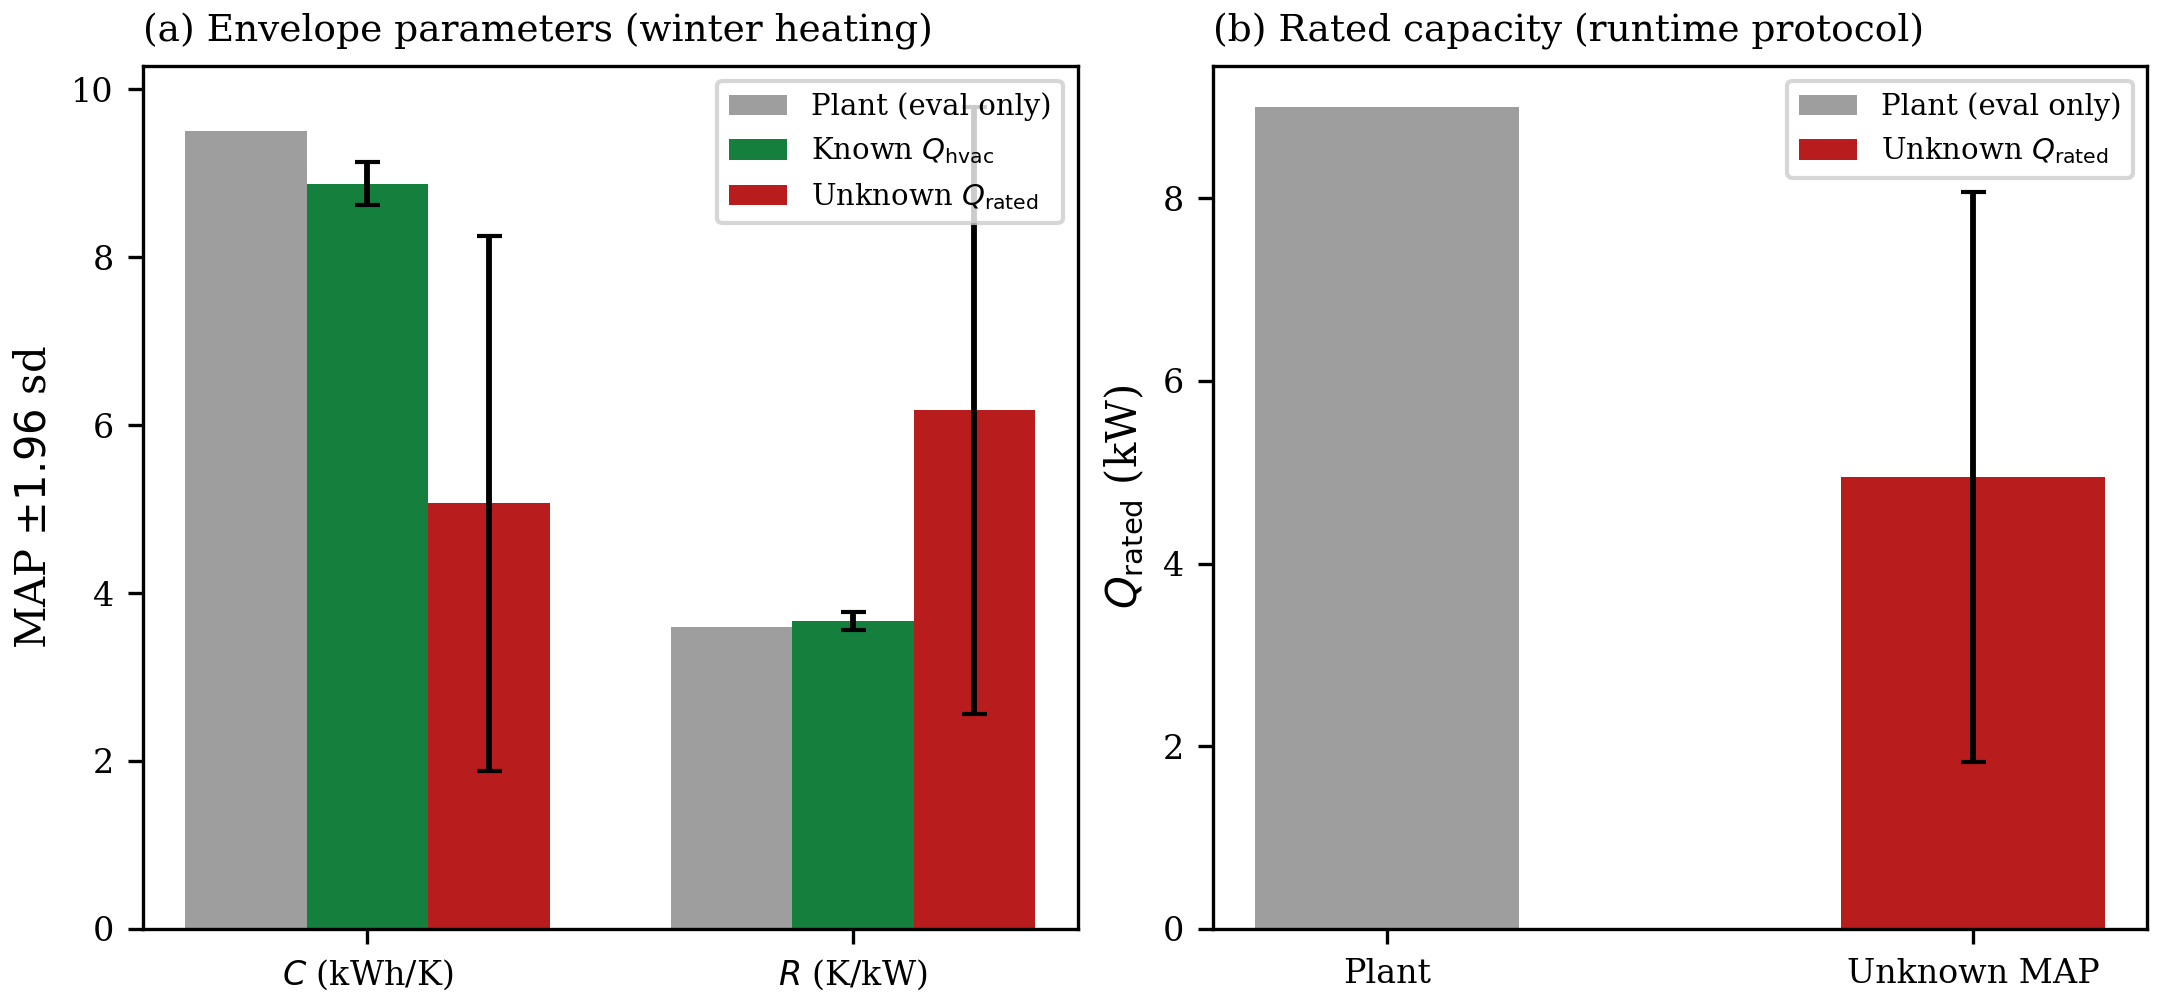
\includegraphics[width=0.92\textwidth]{fig2_params.png}
\caption{\textbf{Winter heating: parameter recovery} under known thermal power (HVAC capacity and on/off states) versus unmetered thermostat runtime. (a) MAP estimates of $C$ and $R$ with Laplace $\pm 1.96\,\mathrm{sd}$ error bars. (b) Estimated rated capacity $Q_\mathrm{rated}$ in the runtime protocol. Metered-power MAP $C$ and $R$ lie near plant truth ($C$ still $\KnownCrel$\% low; its $\pm 1.96\,\mathrm{sd}$ interval misses $C^*$). Runtime alone aliases ($C$ and $Q_\mathrm{rated}$ underestimate truth by $\UnknownCrel$\% and $\UnknownQrel$\%, while $R$ overestimates by $\UnknownRrel$\%).}
\label{fig:params}
\end{figure}

When restricted to observed runtime alone, individual parameters are not recovered: $C=\UnknownC\,\mathrm{kWh/K}$ ($\UnknownCrel$\%), $R=\UnknownR\,\mathrm{K/kW}$ ($\UnknownRrel$\%), and $Q_\mathrm{rated}=\UnknownQ\,\mathrm{kW}$ ($\UnknownQrel$\%). Relative to plant truth, $C$ and $Q_\mathrm{rated}$ scale by $0.53$ and $0.55$ while $R$ expands by $1.72$. That is the direction of~\eqref{eq:aliasing-manifold}, but not the exact map: $1/\alpha_C\approx 1.87$, and $RC=\UnknownRC\,\mathrm{h}$ remains $\UnknownRCrel$\% below $\TrueRC\,\mathrm{h}$.

Composite invariants are closer than the separate parameters:
\begin{itemize}
\item The heating ramp $Q_\mathrm{rated}/C=\UnknownQC\,\mathrm{K/h}$ is within $\UnknownQCrel$\% of $\TrueQC\,\mathrm{K/h}$.
\item The time constant $RC$ is within $\UnknownRCrel$\% of plant truth---better than $C$ or $R$ separately, but not an exact invariant of the fitted point.
\end{itemize}
Laplace sds for the unknown protocol are $\pm\UnknownCsd\,\mathrm{kWh/K}$ on $C$, $\pm\UnknownRsd\,\mathrm{K/kW}$ on $R$, and $\pm\UnknownQsd\,\mathrm{kW}$ on $Q_\mathrm{rated}$. The $\pm 1.96\,\mathrm{sd}$ intervals for $C$ and $Q_\mathrm{rated}$ miss plant truth; the interval for $R$ is wide enough to contain $R^*$ even though the MAP is $\UnknownRrel$\% high. These widths are local curvature around the aliased mode, not a test of structural identifiability.

\begin{figure}[t]
\centering
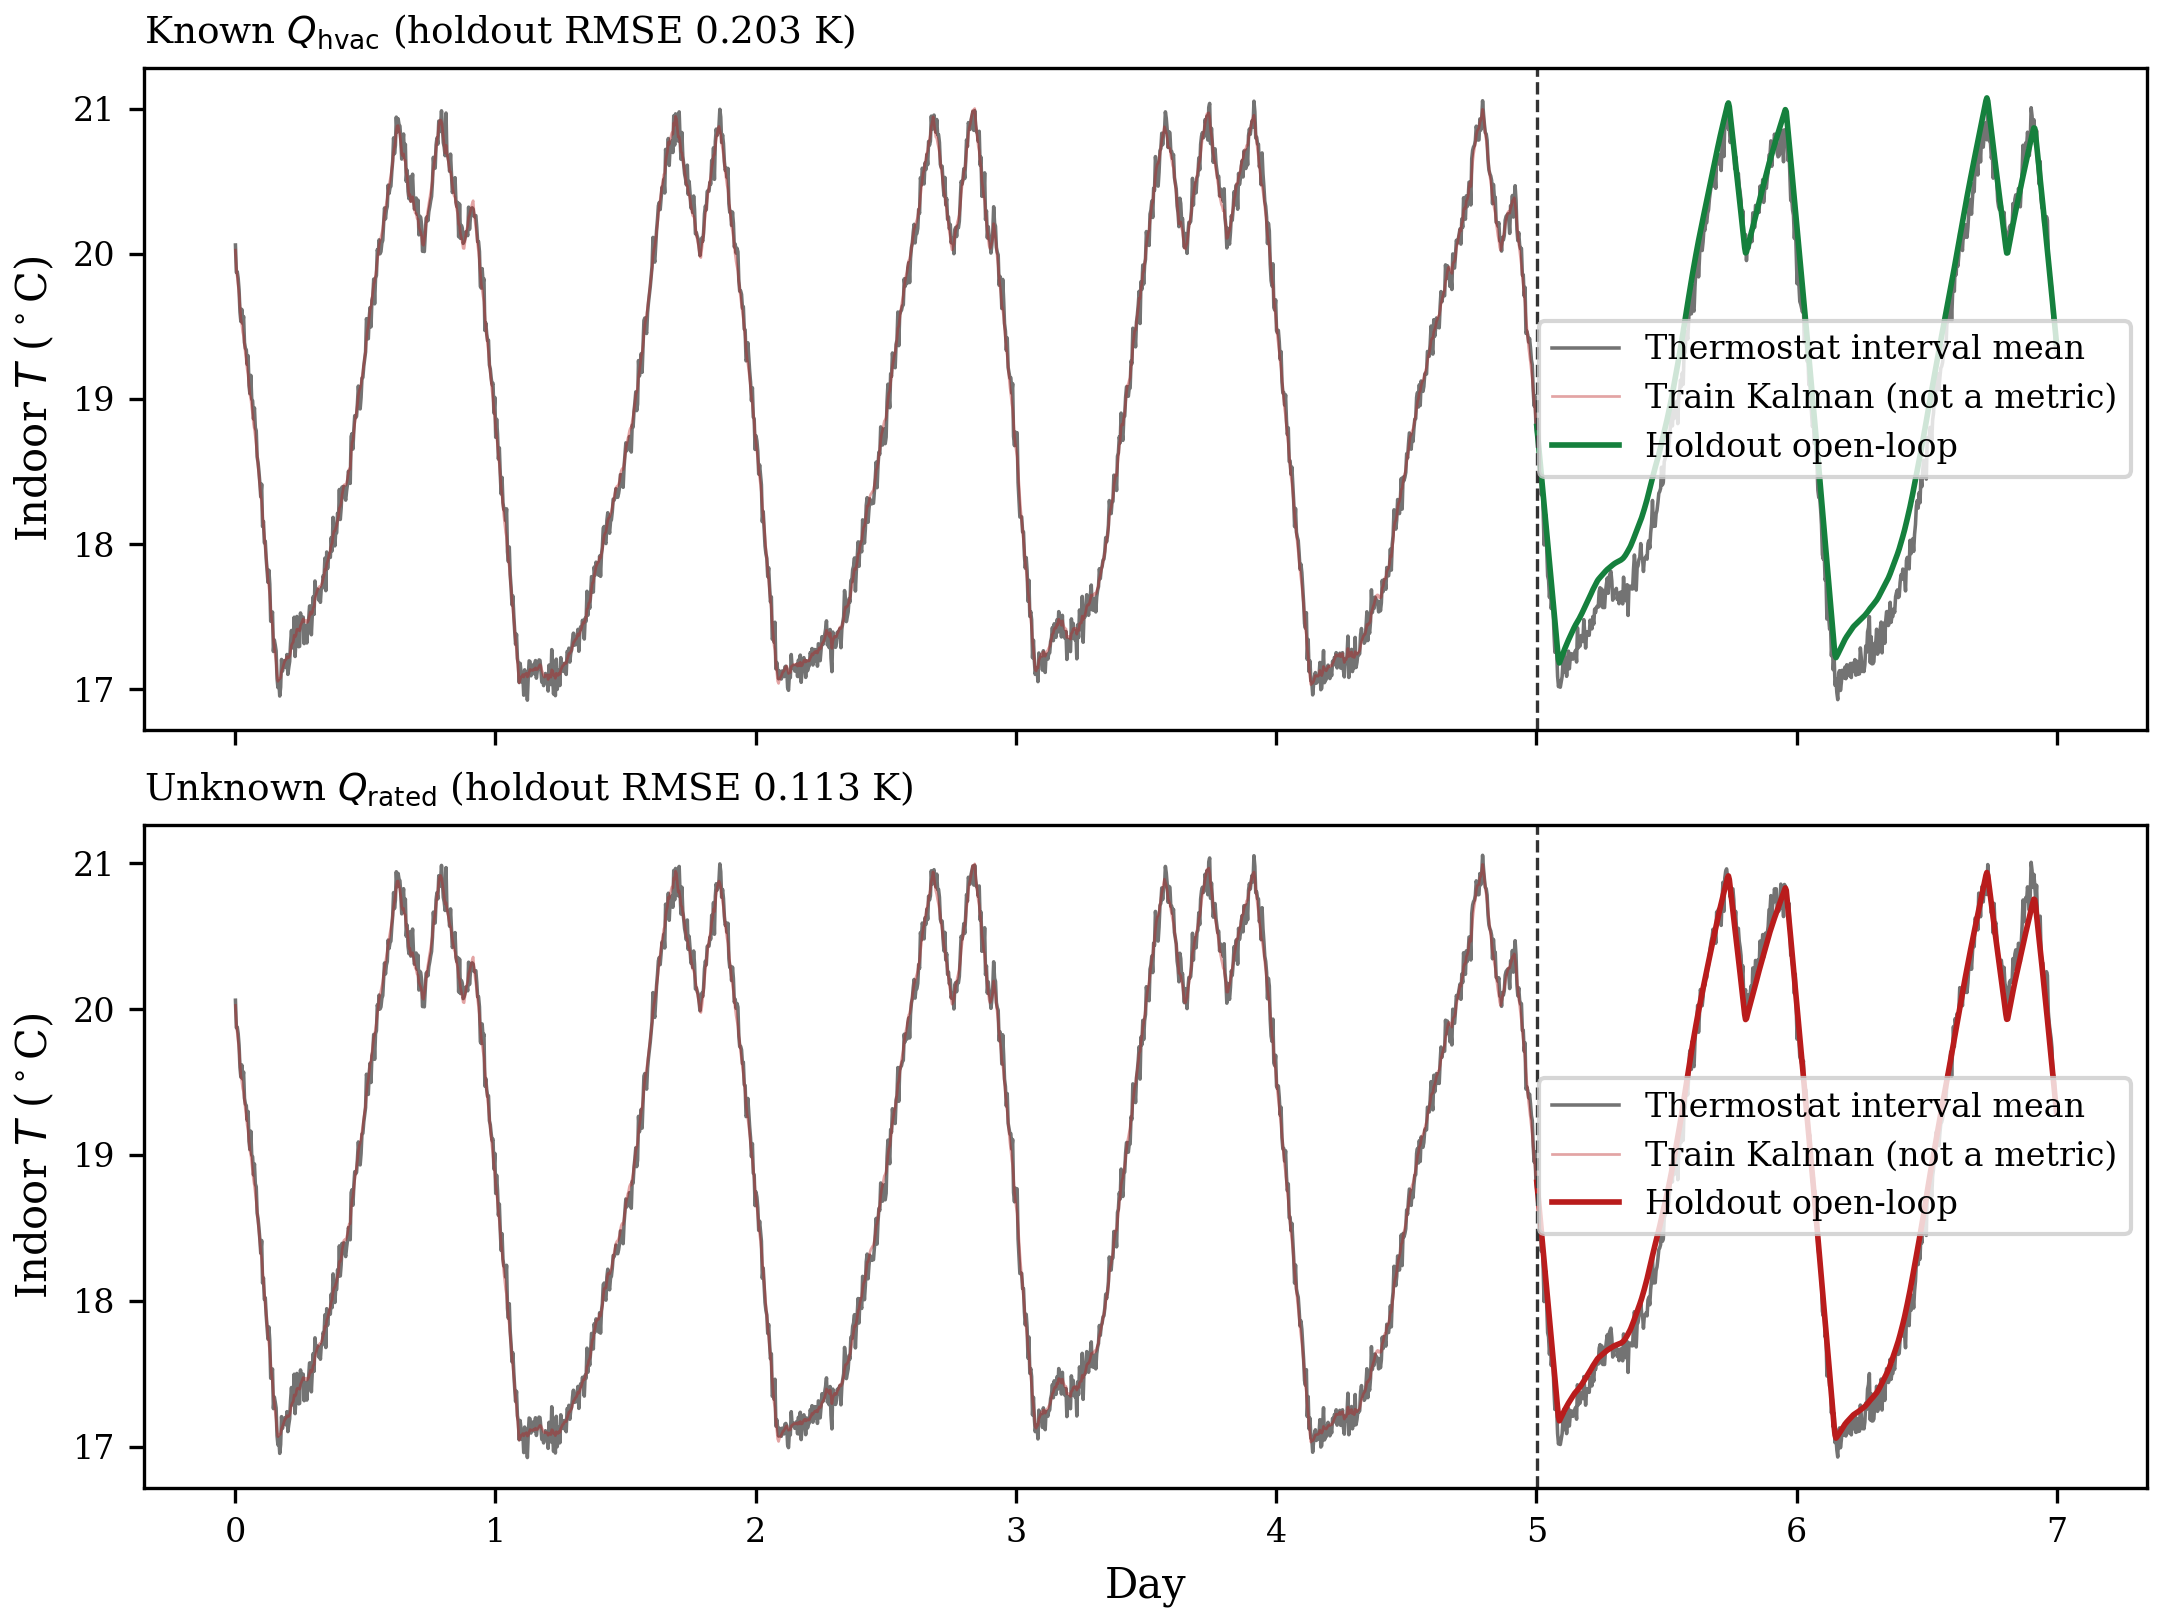
\includegraphics[width=0.92\textwidth]{fig1_holdout.png}
\caption{\textbf{Winter heating: holdout open-loop indoor temperature rollouts.} Top: Known $Q_\mathrm{hvac}$ ($\mathrm{RMSE} = \KnownHoldRMSE\,\mathrm{K}$). Bottom: Unknown $Q_\mathrm{rated}$ runtime ($\mathrm{RMSE} = \UnknownHoldRMSE\,\mathrm{K}$). The dashed line is the 5-day / 2-day chronological split. Solid gray is the thermostat interval mean. The faint red trace is the in-sample train Kalman mean (not a validation metric).}
\label{fig:holdout}
\end{figure}

\begin{figure}[t]
\centering
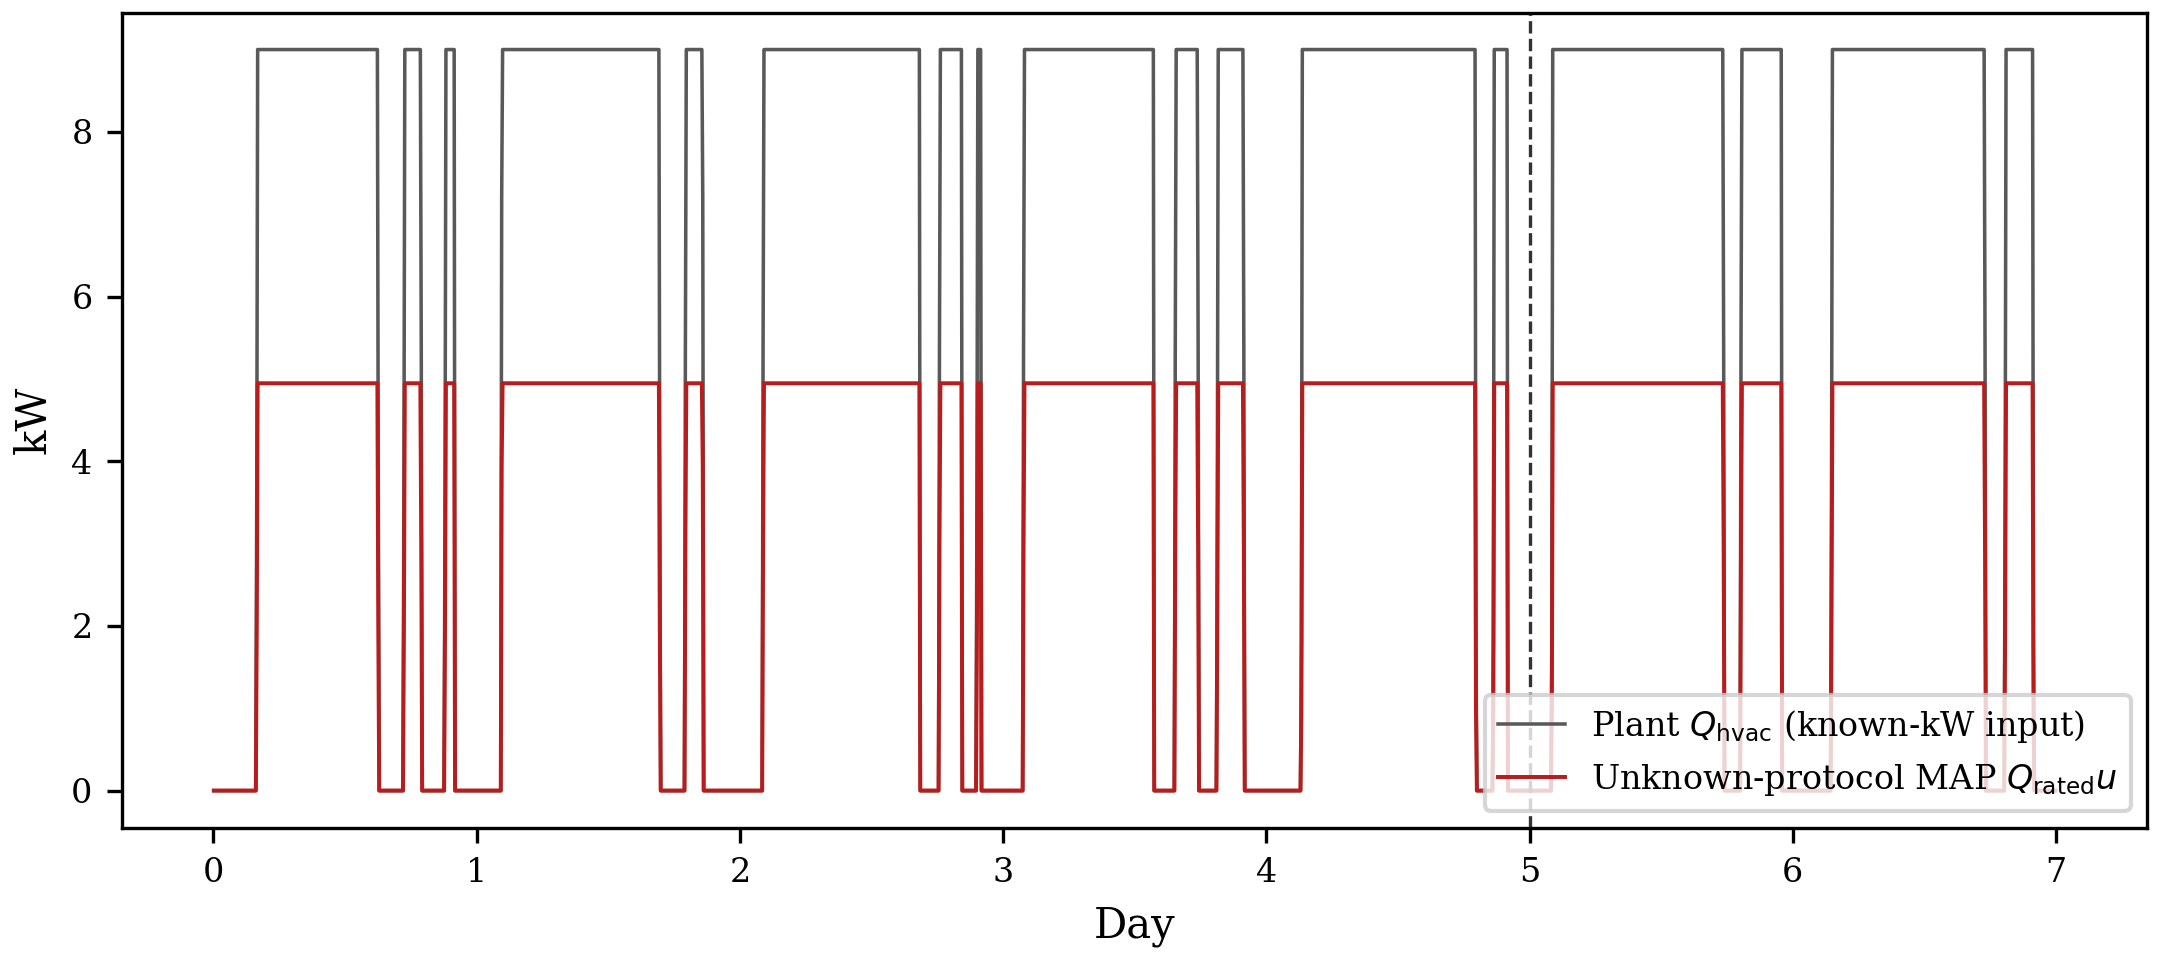
\includegraphics[width=0.92\textwidth]{fig3_hvac.png}
\caption{\textbf{Winter heating: delivered HVAC thermal power.} Solid gray is plant $Q_\mathrm{hvac}(t)$ (known-$Q_\mathrm{hvac}$ input). Red is the runtime-protocol reconstruction $\hat{Q}_\mathrm{rated}u(t)$ ($\hat{Q}_\mathrm{rated} = \UnknownQ\,\mathrm{kW}$). Delivered kW is unobserved during unknown-capacity training.}
\label{fig:hvac}
\end{figure}

\Cref{fig:holdout,fig:hvac} show the winter holdout temperature rollouts and the reconstructed heating power; forecast metrics are discussed jointly with the cooling twin in \Cref{sec:results-holdout}.

\subsection{Summer Cooling Twin}
\label{sec:results-cooling}

\Cref{tab:results-cool} and \Cref{fig:params-cool} repeat the paired protocols on the summer cooling twin. Signed runtime is $u\le 0$; plant $Q_\mathrm{hvac}$ is negative while the compressor is on. The same two-stage schedule, priors, and chronological split are used.

\begin{table}[t]
\caption{\textbf{Summer cooling twin:} paired HVAC-capacity parameter recovery and validation on a seven-day series with a two-day chronological holdout. Relative errors are against the same plant ground truth as \Cref{tab:results}. Rated capacity remains a positive magnitude; cooling enters as $Q_\mathrm{hvac}=Q_\mathrm{rated}u$ with $u\le 0$.}
\label{tab:results-cool}
\centering
\small
\begin{tabular}{@{}lcccc@{}}
\toprule
\textbf{Metric / Parameter} & \textbf{Known $Q_\mathrm{hvac}$} & \textbf{Unknown $Q_\mathrm{rated}$} & \textbf{Plant Truth} & \textbf{Unit} \\
\midrule
Capacitance $C$ & \CoolKnownC\ ($\CoolKnownCrel$\%) & \CoolUnknownC\ ($\CoolUnknownCrel$\%) & \TrueC & $\mathrm{kWh/K}$ \\
Resistance $R$ & \CoolKnownR\ ($\CoolKnownRrel$\%) & \CoolUnknownR\ ($\CoolUnknownRrel$\%) & \TrueR & $\mathrm{K/kW}$ \\
Rated Capacity $Q_\mathrm{rated}$ & Given / Metered & \CoolUnknownQ\ ($\CoolUnknownQrel$\%) & \TrueQrated & $\mathrm{kW}$ \\
Solar Aperture $A_s$ & \CoolKnownAs\ ($\CoolKnownAsrel$\%) & \CoolUnknownAs\ ($\CoolUnknownAsrel$\%) & \TrueAs & $\mathrm{m}^2$ \\
\midrule
Time Constant $RC$ & \CoolKnownRC\ ($\CoolKnownRCrel$\%) & \CoolUnknownRC\ ($\CoolUnknownRCrel$\%) & \TrueRC & $\mathrm{h}$ \\
Cooling Ramp Rate $Q_\mathrm{rated}/C$ & --- & \CoolUnknownQC\ ($\CoolUnknownQCrel$\%) & \TrueQC & $\mathrm{K/h}$ \\
\midrule
Train Mean Kalman NLL & \CoolKnownTrainNLL & \CoolUnknownTrainNLL & --- & $\mathrm{nats}$ \\
Holdout Open-Loop RMSE & \CoolKnownHoldRMSE & \CoolUnknownHoldRMSE & --- & $\mathrm{K}$ \\
Holdout Open-Loop MAE & \CoolKnownHoldMAE & \CoolUnknownHoldMAE & --- & $\mathrm{K}$ \\
\bottomrule
\end{tabular}
\end{table}

\begin{figure}[t]
\centering
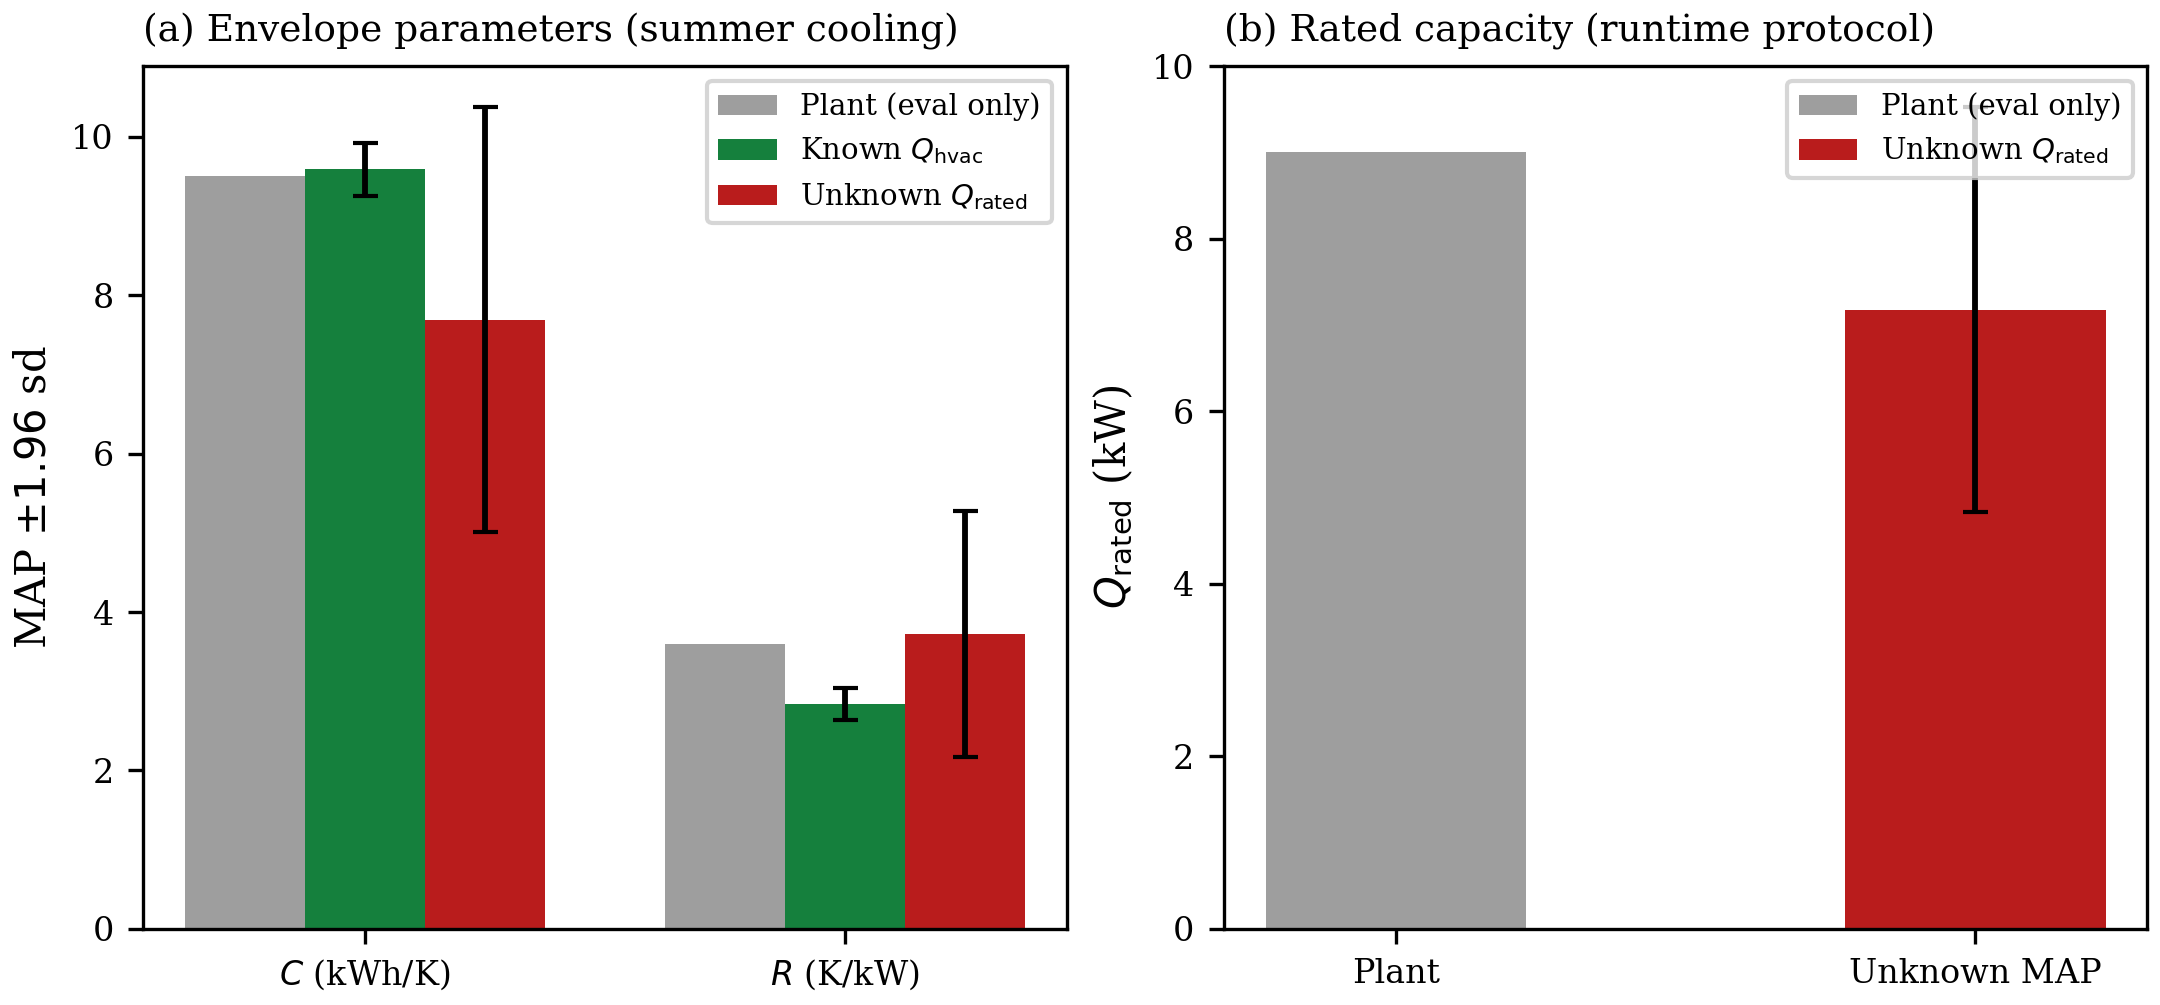
\includegraphics[width=0.92\textwidth]{fig4_params_cool.png}
\caption{\textbf{Summer cooling: parameter recovery} under known delivered power versus unmetered signed runtime. (a) MAP $C$ and $R$ with Laplace $\pm 1.96\,\mathrm{sd}$. (b) Runtime-protocol $Q_\mathrm{rated}$. Metered cooling recovers $C$ tightly; runtime still underestimates $C$ and $Q_\mathrm{rated}$ together while $R$ stays near plant truth. Source: \texttt{paper/figures/fig4\_params\_cool.csv}.}
\label{fig:params-cool}
\end{figure}

Metered cooling power recovers capacitance tightly ($C = \CoolKnownC\,\mathrm{kWh/K}$, $\CoolKnownCrel$\%) and improves solar aperture ($A_s = \CoolKnownAs\,\mathrm{m}^2$, $\CoolKnownAsrel$\%) relative to the winter twin, but envelope resistance is biased ($R = \CoolKnownR\,\mathrm{K/kW}$, $\CoolKnownRrel$\%; $RC = \CoolKnownRC\,\mathrm{h}$, $\CoolKnownRCrel$\%), consistent with a summer trade-off between $UA(T_a-T)$ and $A_s I$. The known-kW $\pm 1.96\,\mathrm{sd}$ interval for summer $R$ does not contain $R^*$ ($z=7.3$). Runtime-only identification does not inflate $R$ as in winter: $R = \CoolUnknownR\,\mathrm{K/kW}$ ($\CoolUnknownRrel$\%) stays near plant truth, while $C = \CoolUnknownC\,\mathrm{kWh/K}$ ($\CoolUnknownCrel$\%) and $Q_\mathrm{rated} = \CoolUnknownQ\,\mathrm{kW}$ ($\CoolUnknownQrel$\%) still scale together ($\alpha_C=0.81$, $\alpha_Q=0.80$). The signed ramp $Q_\mathrm{rated}/C = \CoolUnknownQC\,\mathrm{K/h}$ matches truth to $\CoolUnknownQCrel$\%; $RC = \CoolUnknownRC\,\mathrm{h}$ is off by $\CoolUnknownRCrel$\% because $R$ no longer expands to offset the low $C$. Laplace widths on the runtime mode are large ($\pm\CoolUnknownCsd\,\mathrm{kWh/K}$ on $C$, $\pm\CoolUnknownQsd\,\mathrm{kW}$ on $Q_\mathrm{rated}$); unlike winter, those wide intervals happen to contain plant $C^*$, $R^*$, and $Q_\mathrm{rated}^*$.

\begin{figure}[t]
\centering
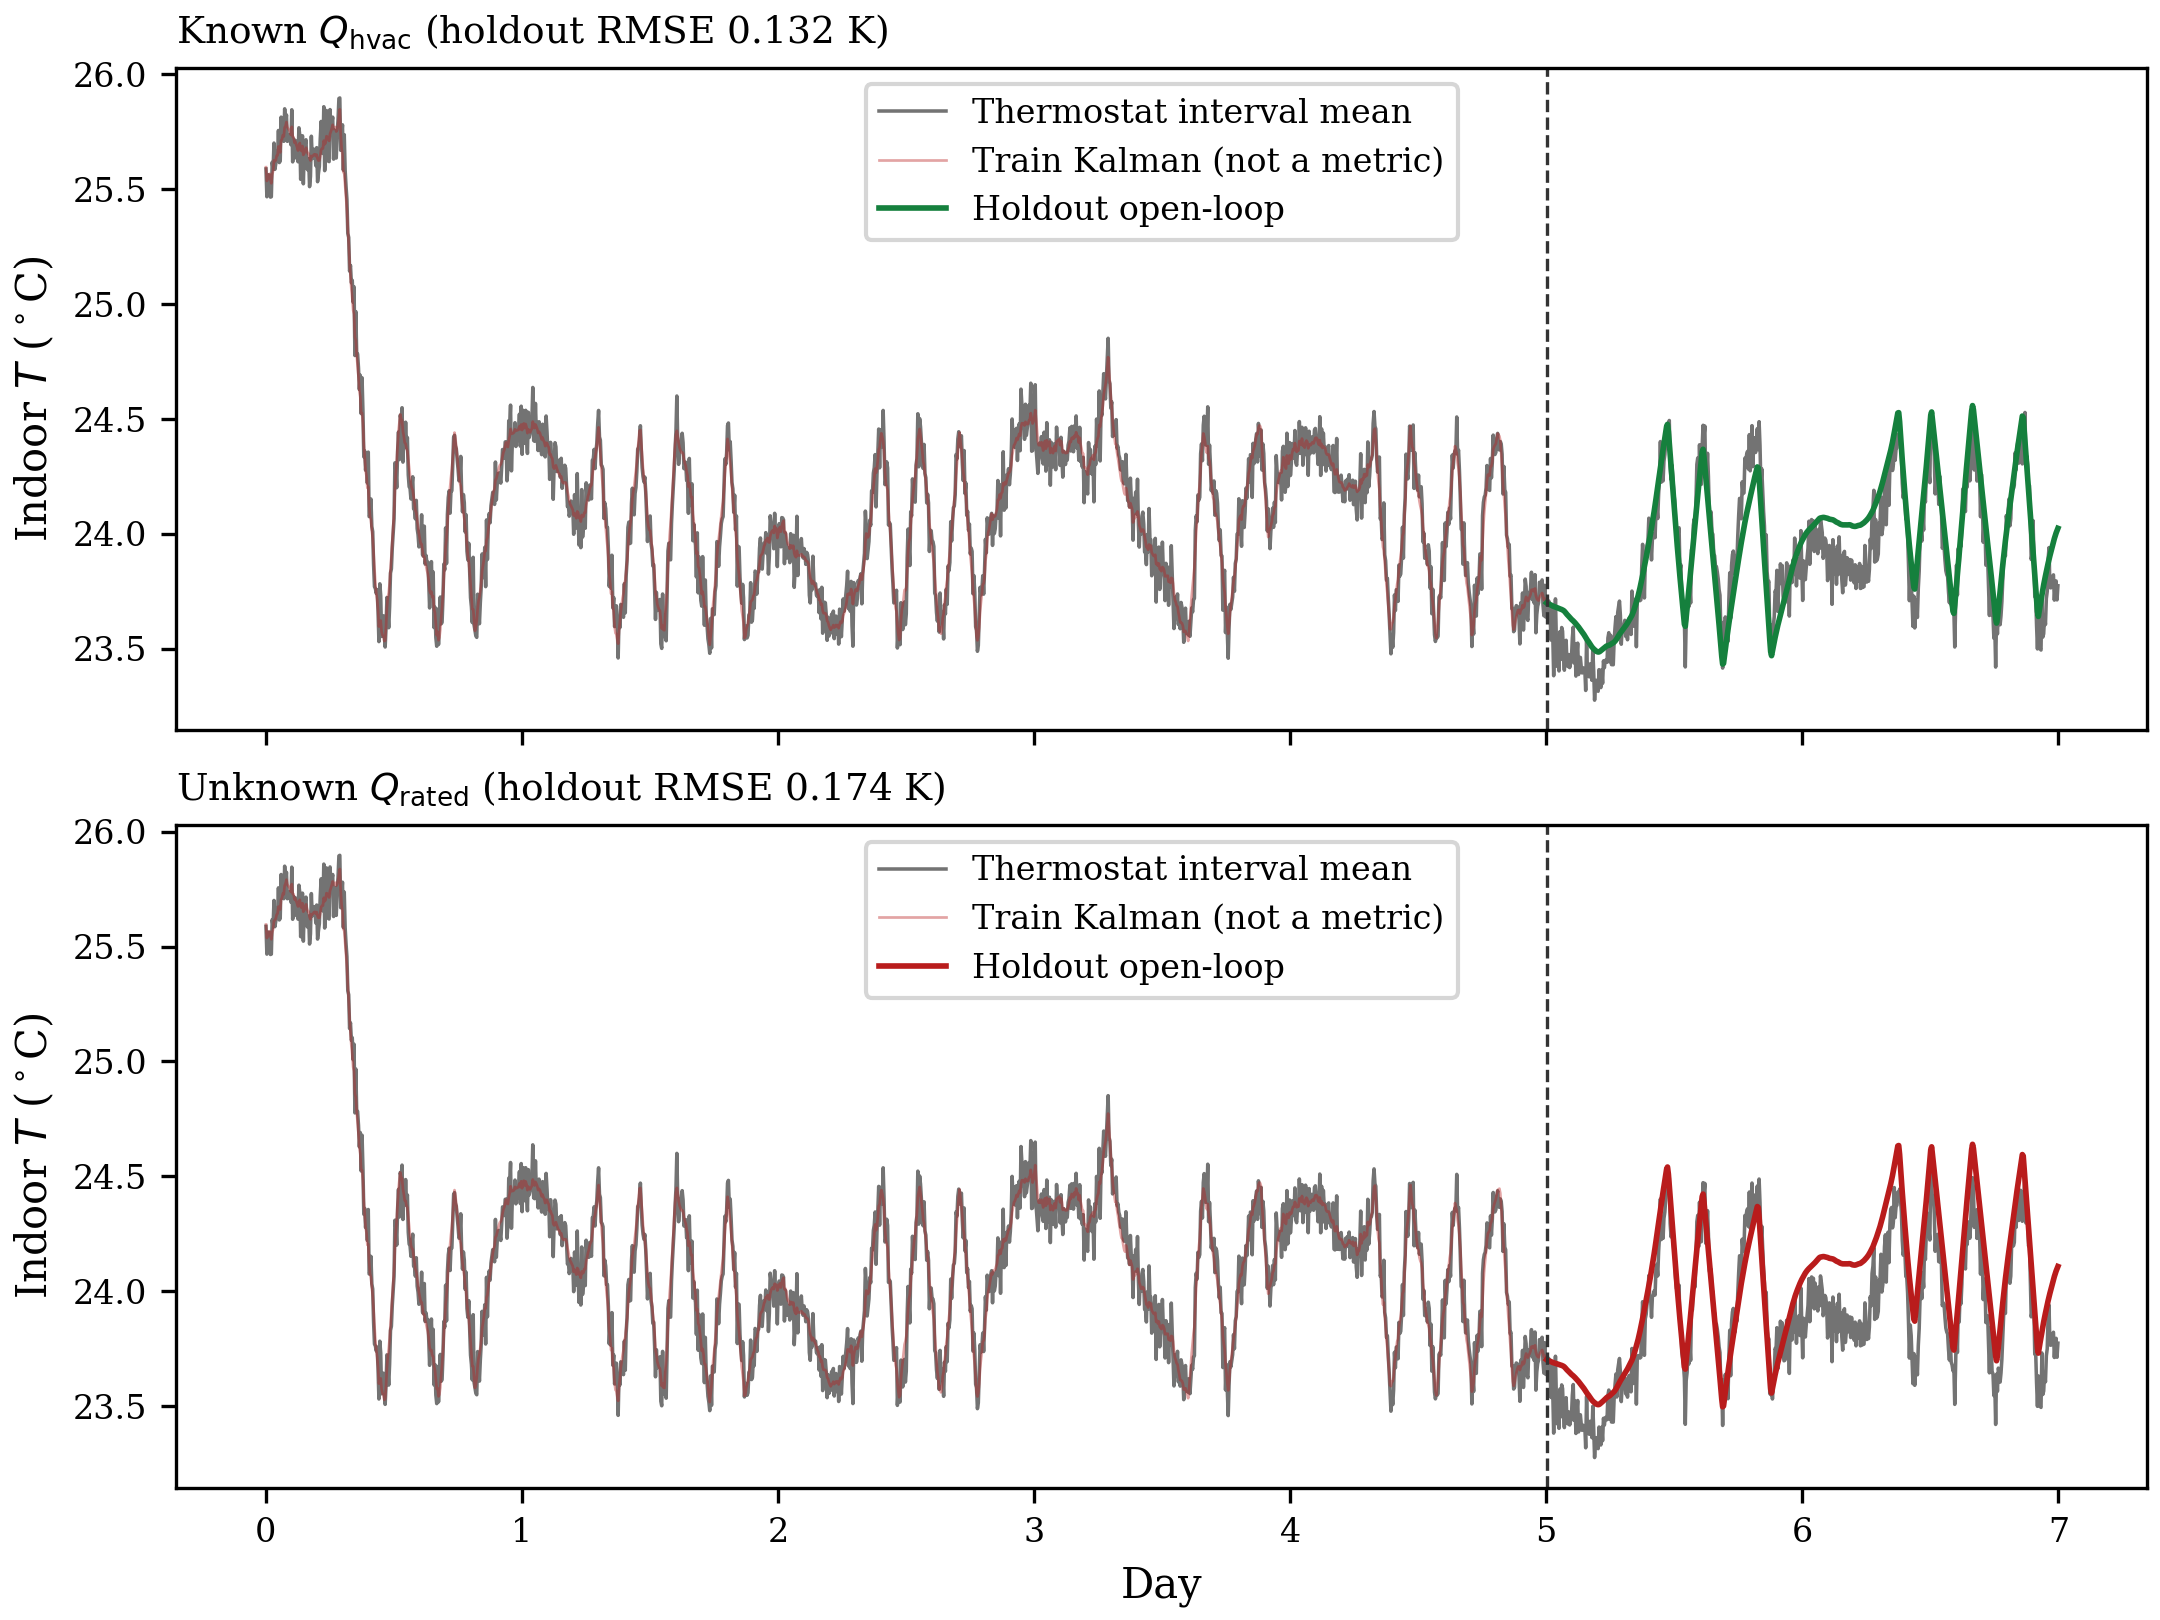
\includegraphics[width=0.92\textwidth]{fig5_holdout_cool.png}
\caption{\textbf{Summer cooling: holdout open-loop indoor temperature rollouts.} Top: Known $Q_\mathrm{hvac}$ ($\mathrm{RMSE} = \CoolKnownHoldRMSE\,\mathrm{K}$). Bottom: Unknown $Q_\mathrm{rated}$ ($\mathrm{RMSE} = \CoolUnknownHoldRMSE\,\mathrm{K}$). Source: \texttt{paper/figures/fig5\_holdout\_cool.csv}.}
\label{fig:holdout-cool}
\end{figure}

\begin{figure}[t]
\centering
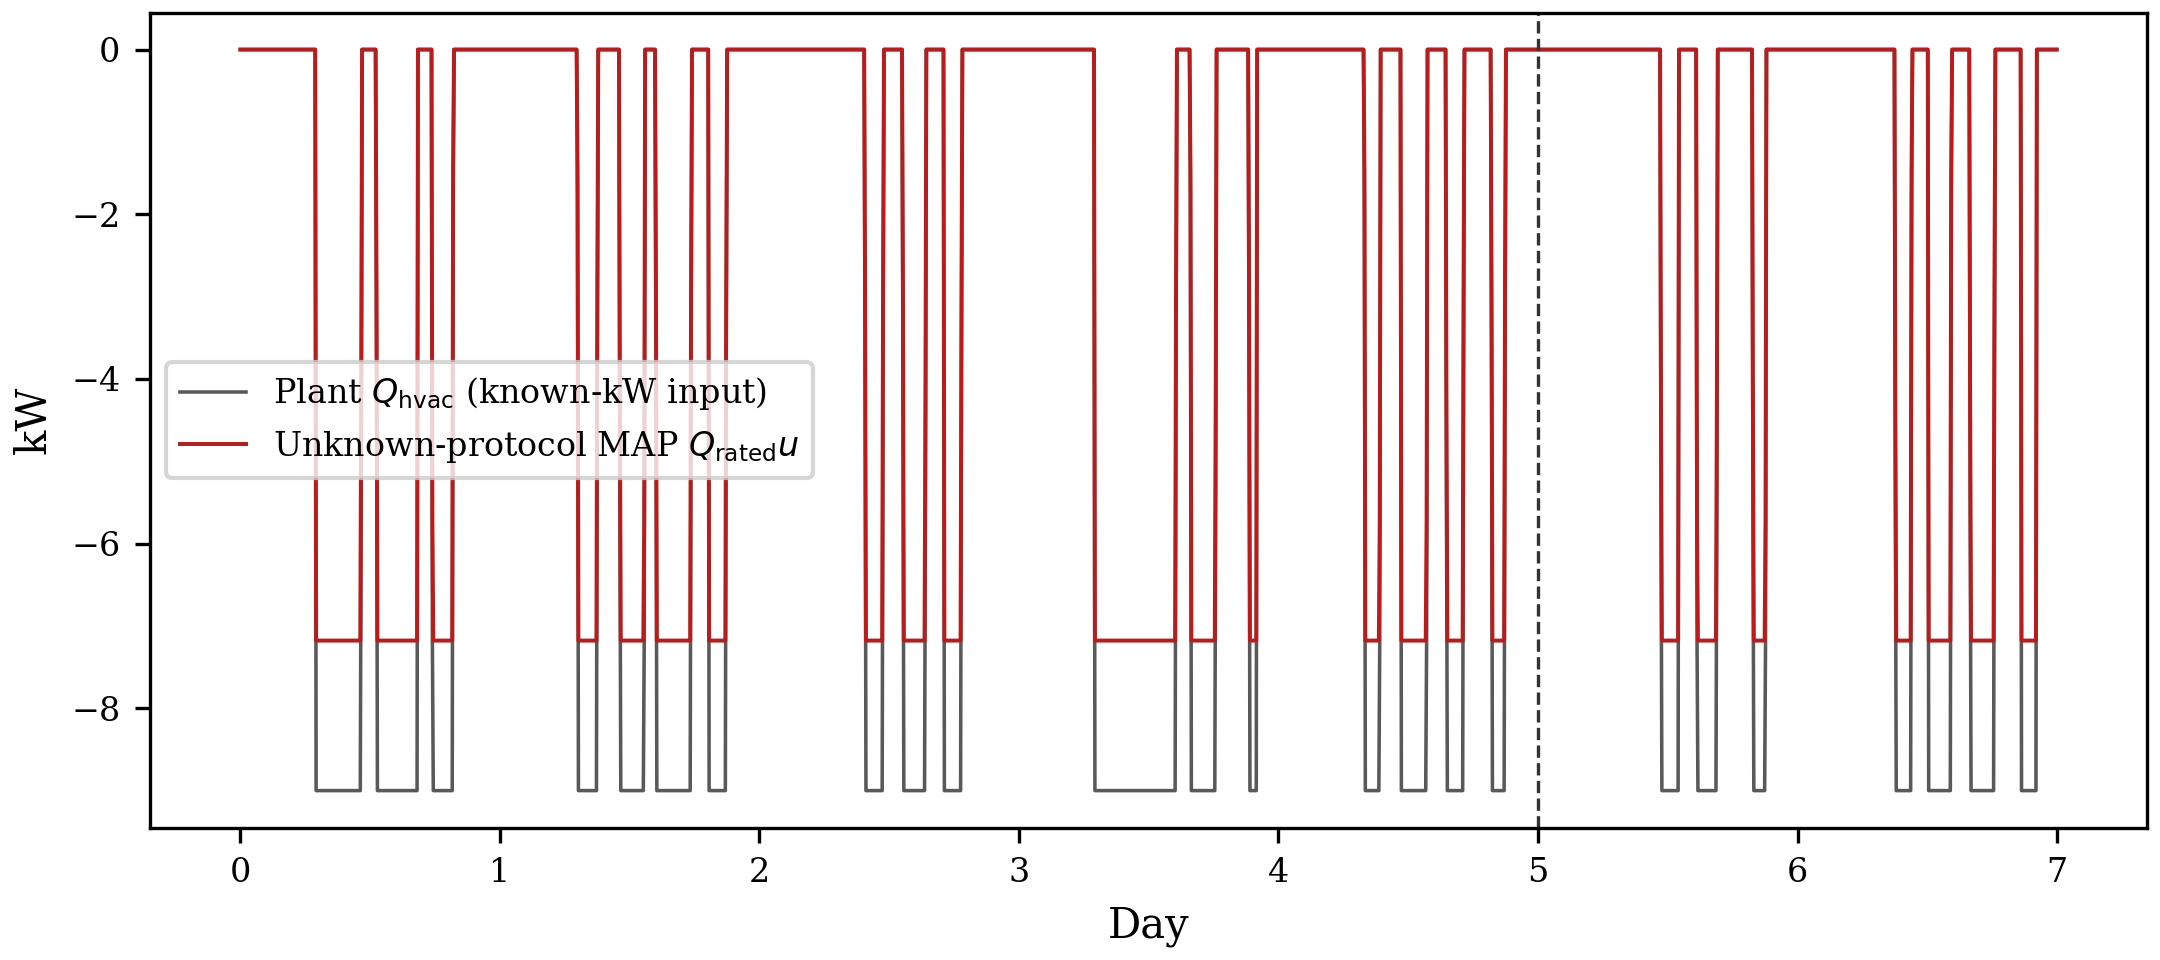
\includegraphics[width=0.92\textwidth]{fig6_hvac_cool.png}
\caption{\textbf{Summer cooling: delivered HVAC thermal power.} Plant $Q_\mathrm{hvac}$ is negative while cooling. Red is $\hat{Q}_\mathrm{rated}u(t)$ from the runtime protocol ($\hat{Q}_\mathrm{rated} = \CoolUnknownQ\,\mathrm{kW}$). Source: \texttt{paper/figures/fig6\_hvac\_cool.csv}.}
\label{fig:hvac-cool}
\end{figure}

\subsection{Holdout Open-Loop Temperature Forecasting}
\label{sec:results-holdout}

\Cref{fig:holdout} displays winter holdout open-loop temperature rollouts, and \Cref{fig:hvac} compares plant heating power against $\hat{Q}_\mathrm{rated}u(t)$. \Cref{fig:holdout-cool,fig:hvac-cool} show the analogous summer traces, with $Q_\mathrm{hvac}<0$ while the compressor runs.

On the winter holdout, known $Q_\mathrm{hvac}$ achieves open-loop RMSE $\KnownHoldRMSE\,\mathrm{K}$ (MAE $\KnownHoldMAE\,\mathrm{K}$) and unknown $Q_\mathrm{rated}$ achieves $\UnknownHoldRMSE\,\mathrm{K}$ (MAE $\UnknownHoldMAE\,\mathrm{K}$). On the summer holdout the corresponding RMSEs are $\CoolKnownHoldRMSE\,\mathrm{K}$ and $\CoolUnknownHoldRMSE\,\mathrm{K}$ (MAE $\CoolKnownHoldMAE\,\mathrm{K}$ and $\CoolUnknownHoldMAE\,\mathrm{K}$). Winter is the sharper forecasting-versus-identification trap: the runtime protocol \emph{beats} metered-power temperature error while its $C$, $R$, and $Q_\mathrm{rated}$ are far from plant truth. Summer is milder: runtime RMSE is slightly worse than metered power, and both summer RMSEs are below $0.2\,\mathrm{K}$ (winter known-kW RMSE is $\KnownHoldRMSE\,\mathrm{K}$). Only the runtime fit jointly biases $C$ and $Q_\mathrm{rated}$ (known-kW summer $C$ error is $\CoolKnownCrel$\%). The summer known-kW fit is a second mismatch: holdout RMSE is $\CoolKnownHoldRMSE\,\mathrm{K}$ while $R$ is $\CoolKnownRrel$\% low. Because the signed ramp $Q_\mathrm{rated}/C$ is close to truth, $\frac{dT}{dt} \approx \frac{Q_\mathrm{rated}}{C}u - \frac{1}{RC}(T - T_a)$ can still produce a plausible trajectory even when $C$ and $Q_\mathrm{rated}$ are individually wrong. The neural remainder and biased parameters adapt to the path likelihood without identifying the underlying physical quantities.

\section{Discussion}
\label{sec:discussion}

\subsection{The Forecasting versus Identification Trap}
\label{sec:discussion-trap}
The central finding of this investigation is that out-of-sample temperature forecasting accuracy is a deceptive metric for physical model identification. In building energy literature, hybrid neural ODEs and PINNs are frequently validated by demonstrating sub-degree Celsius tracking RMSE on validation sets~\cite{gokhale2022,sievers2023}. Our winter results demonstrate that an identified model can achieve exceptional open-loop forecasting accuracy ($\mathrm{RMSE} = \UnknownHoldRMSE\,\mathrm{K}$) while its physical parameters are catastrophically wrong ($C$ biased by $\UnknownCrel$\%, $R$ biased by $\UnknownRrel$\%, and $Q_\mathrm{rated}$ biased by $\UnknownQrel$\%). The summer runtime twin is less extreme on $R$ ($\CoolUnknownRrel$\%) but still aliases $C$ and $Q_\mathrm{rated}$ ($\CoolUnknownCrel$\% / $\CoolUnknownQrel$\%) at a holdout RMSE of $\CoolUnknownHoldRMSE\,\mathrm{K}$. The trap is not confined to unmetered runtime: the summer known-kW fit achieves RMSE $\CoolKnownHoldRMSE\,\mathrm{K}$ with $R$ biased by $\CoolKnownRrel$\%.

This discrepancy has severe practical implications:
\begin{itemize}
\item \textbf{Building Retrofit Auditing:} Using the winter runtime $R = \UnknownR\,\mathrm{K/kW}$ would lead energy auditors to conclude that the envelope is nearly twice as well-insulated as it actually is ($R^* = \TrueR\,\mathrm{K/kW}$), resulting in faulty investment decisions.
\item \textbf{Demand Flexibility and Thermal Battery Sizing:} Using the winter runtime $C = \UnknownC\,\mathrm{kWh/K}$ (or the summer runtime $C = \CoolUnknownC\,\mathrm{kWh/K}$) underestimates thermal storage relative to $C^* = \TrueC\,\mathrm{kWh/K}$, miscalculating how long HVAC loads can be curtailed during peak events.
\item \textbf{Downstream Model Predictive Control:} An MPC controller relying on the aliased parameters could incorrectly schedule pre-heating or pre-cooling duration under variable energy prices, with a risk of comfort violations or sub-optimal energy costs. That downstream control loop is not simulated here.
\end{itemize}

\subsection{Pathways to Reduce Runtime Observability Limits}
\label{sec:discussion-pathways}
To reduce runtime $Q_\mathrm{rated}$--$C$ aliasing (and the winter $R$ expansion that can accompany it) without sub-metering, several strategies are available:
\begin{enumerate}
\item \textbf{Active Excitation and Dedicated Setback Maneuvers:} Passive closed-loop thermostat operation creates high-frequency cycling that obscures thermal inertia. Designing automated grid-interactive excitation maneuvers---such as multi-hour coasting periods ($u = 0$) during mild weather or controlled pre-heating pulses---would provide extended free-response decay data aimed at separating $\tau = RC$ from $Q/C$. These maneuvers were not run on the present twins.
\item \textbf{Informative Bayesian Equipment Priors:} Incorporating prior distributions on $Q_\mathrm{rated}$ derived from HVAC nameplate ratings, manual J load calculations, or conditioned floor area priors ($\sim 50-80\,\mathrm{W\,m}^{-2}$) would be expected to anchor the scaling factor $\alpha$. The weak log-priors used here ($C_0=R_0=Q_0=6$, $\lambda_\mathrm{prior}=0.002$) did not.
\item \textbf{Multi-Modal Telemetry (Smart Meter Disaggregation):} Coupling 5-minute thermostat runtime with whole-home smart meter power data ($P_\mathrm{grid}$) allows non-intrusive load monitoring (NILM) to estimate steady-state electrical power $P_\mathrm{hvac}$, which, combined with nominal heat pump COP curves, bounds $Q_\mathrm{rated}$.
\end{enumerate}

\subsection{Methodological Considerations in Uncertainty Quantification}
\label{sec:discussion-uq}
Our Laplace UQ is a finite-difference Hessian of the train sum-NLL MAP with neural remainder/diffusion weights fixed, plus a positive-definite eigenvalue shift (Section~\ref{sec:id-uq}). Intervals therefore describe local curvature of that conditional objective, not frequentist coverage. On the winter known-kW fit the $C$ interval misses $C^*$ by $4.8$ sd while $R$ is covered. On the summer known-kW fit the $R$ interval misses $R^*$ ($z=7.3$) while $C$ is covered. On winter runtime-only, the $C$ and $Q_\mathrm{rated}$ intervals miss plant truth, but the wide $R$ interval still contains $R^*$. On summer runtime-only the intervals are wide enough to contain $C^*$, $R^*$, and $Q_\mathrm{rated}^*$ even though the MAP for $C$ and $Q_\mathrm{rated}$ is $19$--$20$\% low. Full Bayesian sampling over neural-SDE weights is not implemented here.

\subsection{Limitations and Future Extensions}
\label{sec:discussion-limits}
This study evaluated a single-zone lumped (1R1C-G) thermal representation on paired winter-heating and summer-cooling digital twins. Several physical phenomena remain for future work:
\begin{itemize}
\item \textbf{Higher-Order Thermal Networks (2R2C / Multi-Zone):} Real structures exhibit distinct time constants for indoor air versus heavy structural masonry/concrete envelopes. Extending the differentiable SDE filter to 2R2C formulations is mathematically straightforward within our JAX framework.
\item \textbf{Variable-Capacity Heat Pumps and Defrost Cycles:} In inverter-driven heat pumps, $Q_\mathrm{rated}$ is a dynamic function of outdoor ambient temperature $T_a(t)$ and compressor frequency. Integrating physics-based COP curves into $Q_\mathrm{hvac}(T_a, u)$ will be essential for modern heat-pump retrofits; the cooling twin here still uses a constant rated magnitude.
\item \textbf{Empirical Field Validation:} Validating the PIN-SDE framework on large-scale empirical datasets (e.g., ecobee Donate Your Data) with independent sub-metered validation testbeds is a primary direction for future research.
\end{itemize}

\section{Conclusions}
\label{sec:conclusion}
We have presented a physics-informed neural stochastic differential equation (PIN-SDE) framework that bridges gray-box thermal modeling and smart-thermostat telemetry. By integrating a left-endpoint interval-mean Kalman filter, a latent Ornstein--Uhlenbeck occupancy process, and an identifiability-regularized neural remainder, the model provides an end-to-end differentiable pipeline in JAX for building thermal identification.

Our paired digital-twin experiments in winter heating and summer cooling demonstrate that metered thermal power brings MAP $C$ to $\KnownCrel$\% (heating) and $\CoolKnownCrel$\% (cooling) of plant truth, but it does not identify summer $R$ ($\CoolKnownRrel$\%; holdout RMSE $\CoolKnownHoldRMSE\,\mathrm{K}$). Unmetered runtime aliases $C$ and $Q_\mathrm{rated}$ in both seasons ($\UnknownCrel$\% / $\CoolUnknownCrel$\% on $C$, $\UnknownQrel$\% / $\CoolUnknownQrel$\% on $Q_\mathrm{rated}$). Winter also inflates $R$ by $\UnknownRrel$\%; summer runtime $R$ is within $\CoolUnknownRrel$\% of plant truth but still mis-scales $C$ and $Q_\mathrm{rated}$. The remainder orthogonality penalty and the weak log-priors used here do not break that $Q_\mathrm{rated}$--$C$ aliasing. Runtime-only holdout open-loop temperature RMSE remains low ($\UnknownHoldRMSE\,\mathrm{K}$ heating, $\CoolUnknownHoldRMSE\,\mathrm{K}$ cooling). Temperature prediction accuracy is therefore an insufficient criterion for physical parameter identification. Informative capacity priors or dedicated excitation were not tested here; they are the natural next constraints if the goal is to pin down $C$ and $Q_\mathrm{rated}$ from runtime.

\section*{Materials and Methods}
\label{sec:methods}
The identification framework is implemented in Python~3.10+ using JAX~\cite{bradbury2018}, Optax Adam (global-norm clip $5$), and NumPy/Matplotlib. The interval-average Kalman filter and mean open-loop rollout use \path{jax.lax.scan}. Training gradients use \path{jax.grad}. The Laplace Hessian is a finite-difference of those gradients, not \path{jax.hessian}. Reproduction is \path{scripts/generate_paper_figures.py} (synthetic seed $0$, \texttt{TrainConfig} seed $1$). Source is released under the MIT License~\cite{yang2026pinde}.

\section*{Data Availability}
The synthetic time series are generated with seed $0$ by \path{pi_nsde_building_thermal.synthetic}. Identifier initialization and Adam use \texttt{TrainConfig.seed}${}=1$. Fitted MAP values, Laplace sds, and holdout RMSE/MAE are those written by \path{scripts/generate_paper_figures.py} to \path{paper/figures/manifest.json} and \path{paper/generated_numbers.tex}.

\section*{Code Availability}
The complete software package, including model architectures, Kalman filter implementations, training pipelines, and plotting scripts, is publicly available on GitHub \cite{yang2026pinde}.

\section*{Author Contributions}
\textbf{Sam Yang}: Conceptualization, Methodology, Software, Formal analysis, Investigation, Data curation, Writing -- original draft, Writing -- review \& editing, Visualization. \textbf{Jessica Moorefield}: Investigation, Writing -- review \& editing. Both authors read and approved the final manuscript.

\section*{Generative-AI Disclosure}
During the preparation of this manuscript, the authors utilized large language models (LLMs) to assist with text editing, polishing, and LaTeX formatting. The authors thoroughly verified all mathematical formulations, derivations, software implementations, and numerical results against the codebase outputs. The authors take full responsibility for the contents and conclusions of the paper.

\section*{Competing Interests}
The authors declare no competing financial or non-financial interests.

\section*{Funding and Acknowledgments}
This research was supported in part by Florida State University's Undergraduate Research Opportunity Program (UROP). The authors gratefully acknowledge the open-source software contributions of the JAX and Python scientific computing communities~\cite{bradbury2018}.

\section*{Disclaimer}
The views, opinions, and findings contained in this paper are those of the authors and should not be construed as an official position, policy, or decision of the Center for Advanced Power Systems, Florida State University, the Georgia Institute of Technology, or North Carolina State University.

\bibliographystyle{IEEEtran}
\bibliography{references}

\end{document}
